\chapter{Vektorielle Geometrie}
\chapterauthor{Pascal}
\section{Vektoren}

    \begin{Definition}
        Ein Vektor ist Element eines Vektorraums.
    \end{Definition}\\
    \paragraph{} Vektorräume, wir erinnern uns zurück. Verknüpfungen, inverse Elemente und die dazugehörenden Gesetze, konsequente Definitionen und
    mathematische Korrektheit, die guten alten Zeiten...\\
    Tatsächlich kann ein Vektor in den meisten Fällen als Verschiebung bezeichnet werden, \textbf{nicht aber als Pfeil oder Strich!}\\


    \subsection{Besondere Vektoren}
      \begin{Definition}[- Der Ortsvektor]
        Der Vektor von $O$ auf den Punkt $P$, geschrieben als $\vv{OP}$ oder $\vv{p}$.\\
        Hat $P$ die Koordinaten $(P_1|P_2|...|P_n)$, so besitzt $\vv{p}$ die Darstellung $\left(\begin{array}{c} P_1 \\ P_2 \\ ...\\P_n\end{array}\right)$.
      \end{Definition}

      \begin{Definition}[- Der Nullvektor]
        Der Vektor mit Wert $\left(\begin{array}{c} 0 \\ 0 \\ ...\\0\end{array}\right)$, er hat keine und alle Richtungen zugleich.
      \end{Definition}
      \begin{Bemerkung}
        Er ist somit das neutrale Element der Vektoraddition.
      \end{Bemerkung}

      \begin{Definition}[- Der Verbindingsvektor]
        Der Vektor $\vv{AB}$ ist der Vektor, der den Punkt $A$ auf den Punkt $B$ abbildet. Er ist definiert als:\\ $\vv{AB}=\vv{OB}-\vv{OA}$,
        woraus folgt, dass: \begin{center} $\vv{AB} = \left(\begin{array}{c} b_1 - a_1 \\ b_2 - a_2 \\ ... \\ b_n - a_n \end{array}\right)$. \end{center}
      \end{Definition}

      \begin{Definition}[- Der Gegenvektor]
        Der Gegenvektor zu $\vv{AB}$ ist $\vv{BA}$, definiert als  $-\vv{AB}$.\\

      \end{Definition}

      \begin{Bemerkung}
        Er ist somit das inverse Element der Vektoraddition.
      \end{Bemerkung}

      \begin{Bemerkung}
        \begin{Definition}[- Norm eines Vektors]
        Die Norm eines Vektors ist anschaulich als seine Länge zu interpretieren. Der Betrag, wie sie ebenfalls genannt wird, eines
         Vektors $\vv{v}$ ist folgendermaßen definiert: $\text{|}\vv{v}\text{|} = \sqrt{\displaystyle\sum_{i=1}^{n}v_{i}^2} ; \vv{v}\in\R^n$.
        \end{Definition}
        \begin{minipage}{0.5\textwidth}
          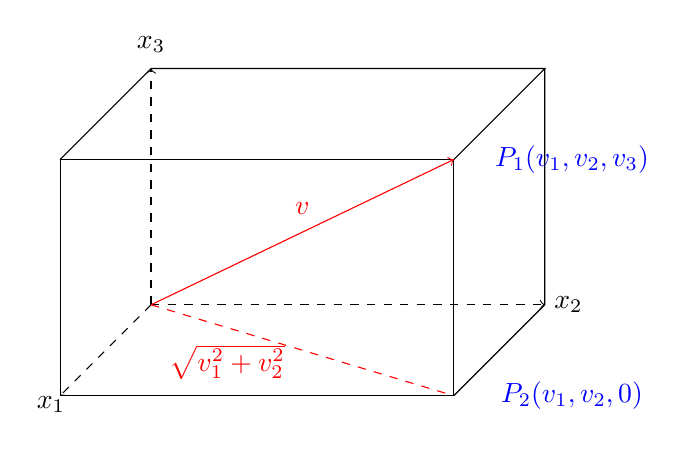
\begin{tikzpicture}
            \draw[dashed, ->] (0,0,0) -- (0,0,3);
            \draw[dashed, ->] (0,0,0) -- (5,0,0);
            \draw[dashed, ->] (0,0,0) -- (0,3,0);
            \draw[dashed, color=red] (0,0,0) -- (5,0,3);
            \draw (0,0,3) -- (5,0,3) -- (5,3,3) -- (0,3,3) -- (0,0,3);
            \draw (0,3,3) -- (0,3,0) -- (5,3,0) -- (5,3,3);
            \draw (5,3,0) -- (5,0,0) -- (5,0,3);
            \draw[->, color=red] (0,0,0) -- (5,3,3);
            \draw (0,0,3.3) node {$x_1$};
            \draw (5.3,0,0) node {$x_2$};
            \draw (0,3.3,0) node {$x_3$};
            \draw (2.5,1.8,1.5) node [color=red]{$\vv{v}$};
            \draw (6.5,3,3) node [color=blue]{$P_1 (v_1, v_2, v_3)$};
            \draw (6.5,0,3) node [color=blue]{$P_2 (v_1, v_2, 0)$};
            \draw (1.7,0,1.9) node [color=red]{$\sqrt{v_1^{2}+v_2^{2}}$};
            \end{tikzpicture}
        \end{minipage}
        \begin{minipage}{0.5\textwidth}
          Anhand dieser Graphik lässt sich die Berechnung der Norm eines Vektors $\vv{v}\in\R^3$ verdeutlichen. Für diesen glit:
          $\text{|}\vv{v}\text{|}=\sqrt{v_1^{2}+v_2^{2}+v_3^{2}}$.
        \end{minipage}
      \end{Bemerkung}

      \begin{Definition}[- Der Einheitsvektor]
        Ein Vektor, dessen Norm 1 beträgt wird als normiert oder Einheitsvektor bezeichnet. Für jeden Vektor $\vv{v}\in\R^{3}$ existiert ein Einheitsvektor $\vv{v^{*}}$ , der folgendermaßen definiert wird: $\vv{v^{*}}=\dfrac{1}{\text{|}\vv{v}\text{|}}*\vv{v}$.
      \end{Definition}




\section{Basen und Erzeugendensystem}

    \begin{Definition}
      Eine endliche Anzahl von Vektoren $\vv{a_1},\vv{a_2},...,\vv{a_n}\in V$ heißt Erzeugendensystem, wenn sich \texbf{jeder} Vektor $\vv{v}\in V$
      als Linearkombination dieser Vektoren schreiben lässt. Um ein Erzeugendensystem zu bilden benötigt man mindestens die Anzahl Vektoren, die der Anzahl von Dimensionen von $\vv{v}$ entspricht. Wenn man \textbf{genau} diese Anzahl besitzt, spricht man von einer Basis.
    \end{Definition}

    \subsection{Besondere Basen}


        \begin{Definition}[- Orthogonalbasis]
          Sind die Vektoren der Basis paarweise orthogonal zueinander, so spricht man von einer \textbf{Orthogonalbasis}.
        \end{Definition}



        \begin{Definition}[- Orthonormalbasis]
          Sind die Vektoren zusätzlich zu dieser Bedingung normiert, wird sie als \textbf{Orthonormalbasis} bezeichnet.
          Die einfachste und meist benutzte Basis des $\R^3$ besteht aus den drei Vektoren $\vv{e_1}=\left(\begin{array}{c}{1\\0\\0}\end{array}\right),
          \vv{e_2}=\left(\begin{array}{c}{0\\1\\0}\end{array}\right),\vv{e_3}=\left(\begin{array}{c}{0\\0\\1}\end{array}\right)$. Sie wird als \textbf{Standardbasis}
          des $\R^3$ bezeichnet. Vektoren wie $\vv{v}=\left(\begin{array}{c}{2\\3\\8}\end{array}\right)$ lassen sich als eine Linearkombination der drei
          Vektoren der Standardbasis darstellen: $\vv{v}=2\cdot\vv{e_1}+3\cdot\vv{e_2}+8\cdot\vv{e_3}$.
        \end{Definition}


    \subsection{Basistransformation}

        \paragraph{} Bilden die Vektoren $\vv{a_1},\vv{a_2},...,\vv{a_n}$ eine Basis des $n$-dimensionalen Vektorraums $V$ und sei der Vektor
         $\vv{v}=\left(\begin{array}{c}{v_1\\v_2\\...\\v_n}\end{array}\right);\vv{v}\in V$. Dann gilt wie üblich:
         $\vv{v}=v_1\cdot\vv{a_1}+v_2\cdot\vv{a_2}+...+v_n\cdot\vv{a_n}$. Sei eine weitere Basis $\vv{b_1},\vv{b_2},...,\vv{b_n}$ des selben Vektorraumes,
          so besitzt der Vektor $\vv{v}$ andere Koordinaten: $\vv{v}=\left(\begin{array}{c}{v'_1\\v'_2\\...\\v'_n}\end{array}\right)$.
          Dabei muss gelten: $\vv{v}=v_1\cdot\vv{a_1}+v_2\cdot\vv{a_2}+...+v_n\cdot\vv{a_n}=v'_1\cdot\vv{b_1}+v'_2\cdot\vv{b_2}+...+v'_n\cdot\vv{b_n}$.
        \\
        \begin{Bemerkung}
            \\
            Um die Koordinaten eines Vektors in einer anderen Basis als der Aktuellen zu bestimmen, löst man diese Gleichung, die sich ergibt.
        \end{Bemerkung}

        \begin{Beispiel}
            Basis 1: Standardbasis des $\R^3$, Basis 2:
            $\vv{b_1}=\left(\begin{array}{c}{4\\9\\-1}\end{array}\right), \vv{b_2}=\left(\begin{array}{c}{-2\\-2\\8}\end{array}\right),
            \vv{b_3}=\left(\begin{array}{c}{1\\3\\1}\end{array}\right)$, Vektor $\vv{v}=\left(\begin{array}{c}{-5\\3\\2}\end{array}\right)$ (in der Standardbasis des $\R^3$)
            \\
            $\vv{v}=-5\cdot\vv{a_1}+3\cdot\vv{a_2}+2\cdot\vv{a_3}=r\cdot\vv{b_1}+s\cdot\vv{b_2}+t\cdot\vv{b_3}$
            $\Leftrightarrow \begin{vmatrix}4r & -2s & t & = & -5 \\
                                            9r & -2s & 3t & = & 3 \\
                                            -r & 8s & t & = & 2
                            \end{vmatrix}
             \\
             \\
             \Leftrightarrow \begin{vmatrix}-r & 8s & t & = & 2 \\
                                            0 & 30s & 5t & = & 3 \\
                                            0 & 70s & 12t & = & 21
                             \end{vmatrix}
             \\
             \\
             \Leftrightarrow \begin{vmatrix}-r & 8s & t & = & 2 \\
                                            0 & 30s & 5t & = & 3 \\
                                            0 & 0 & \frac{1}{3}\cdot t & = & 14
                             \end{vmatrix}
             \\
             \\
             \Leftrightarrow \begin{vmatrix}r & = & -15.2 \\
                                            s & = & -6.9 \\
                                            t & = & 42
                             \end{vmatrix}
            \\
            \\
            \mathbb{L}=\{ -15.2|-6.9|42 \}$
            \\
            Daraus lässt sich folgern: $\vv{v}=-15.2\cdot\vv{b_1}-6.9\cdot\vv{b_2}+42\cdot\vv{b_3}=\left(\begin{array}{c}{-15.2\\-6.9\\42}\end{array}\right)$
             (in der anderen Basis).
            \\

        \end{Beispiel}



\section{Winkel zwischen Vektoren}

    \begin{Definition}
        \paragraph{} Unter einem Winkel zwischen zwei Vektoren versteht man den Winkel, der ensteht, wenn man beide Vektoren an einen \textbf{gemeinsamen Startpunkt}
        verschiebt ohne dabei ihre Ausrichtung zu verändern.
    \end{Definition}


    \subsection{Orientierte Winkel}
        Wenn man in der Mathematik mit Winkeln arbeitet, werden sie immer im \textbf{mathematisch positiven} Sinn angegeben.
        Dies bedeutet, dass man von einem Vektor oder Schenkel, der an den Winkel grenzt, ausgeht und über Rotation um den Schnittpunkt \glqq gegen
        den Uhrzeigersinn\grqq \,zum anderen gelangt, bis beide übereinanderliegen (wenn man davon ausgeht, dass sich beide schneiden).\\
        \begin{minipage}{0.5\textwidth}
          \definecolor{qqwuqq}{rgb}{0,0.4,0}
          \definecolor{ududff}{rgb}{0.3,0.3,1}
          \begin{tikzpicture}[>=triangle 45]
              \draw [line width=0.8pt,color=qqwuqq,fill=qqwuqq,fill opacity=0.1] (0,0) -- (1.3,-0.75) arc (-30:30:1.5) -- cycle;
              \draw [->,line width=0.8pt,color=qqwuqq] (1.3,-0.75) arc (-30:30:1.5);
              \draw [->,line width=0.8pt] (0,0) -- (5.2,3);
              \draw [->,line width=0.8pt] (0,0) -- (5.2,-3);
              \draw [fill=ududff] (5.2,3) circle (1.5pt);
              \draw[color=ududff] (5.4,3.2) node {$A$};
              \draw [fill=ududff] (0,0) circle (1.5pt);
              \draw[color=ududff] (-0.3,0.1) node {$B$};
              \draw [fill=ududff] (5.2,-3) circle (1.5pt);
              \draw[color=ududff] (5.4,-3.2) node {$C$};
              \draw[color=qqwuqq] (0.9,0) node {$\alpha$};
              \draw[color=black] (2.6,-1.7) node {$c$};
              \draw[color=black] (2.6,1.7) node {$a$};
          \end{tikzpicture}
        \end{minipage}
        \begin{minipage}{0.5\textwidth}
          \definecolor{ududff}{rgb}{0.3,0.3,1}
          \definecolor{adadff}{rgb}{0.8,0.8,0}
          \begin{tikzpicture}[>=triangle 45]
              \draw [line width=0.8pt,color=adadff,fill=adadff,fill opacity=0.1] (0,0) -- (1.3,-0.75) arc (-30:30:1.5) -- cycle;
              \draw [<-,line width=0.8pt,color=adadff] (1.3,-0.75) arc (-30:30:1.5);
              \draw [->,line width=0.8pt] (0,0) -- (5.2,3);
              \draw [->,line width=0.8pt] (0,0) -- (5.2,-3);
              \draw [fill=ududff] (5.2,3) circle (1.5pt);
              \draw[color=ududff] (5.4,3.2) node {$A$};
              \draw [fill=ududff] (0,0) circle (1.5pt);
              \draw[color=ududff] (-0.3,0.1) node {$B$};
              \draw [fill=ududff] (5.2,-3) circle (1.5pt);
              \draw[color=ududff] (5.4,-3.2) node {$C$};
              \draw[color=qqwuqq] (0.9,0) node {$\alpha$};
              \draw[color=black] (2.6,-1.7) node {$c$};
              \draw[color=black] (2.6,1.7) node {$a$};
          \end{tikzpicture}
        \end{minipage}

        So ergibt sich $\alpha = \angle ABC = \angle ac = (\vv{BA},\vv{BC}) = \frac{\pi}{3}$. Ein Winkel $\alpha$ wird zudem immer so angegeben, dass $\alpha\in I; I = [-\pi,\pi]$ gilt.
        Dies bedeutet, dass man nur Winkel zwischen $0°$ und $180°$ erhält, und das in beide \glqq Richtungen\grqq, als im mathematisch positiven und negativen Sinn.
        Diese Einschränkung kennzeichnet man mit dem Ausdruck \glqq \textbf{modulo $2\pi$}\grqq.


    \subsection{Rechnungen mit Winkeln}

        \paragraph{} Bei Berechnungen von Winkeln zwischen Vektoren geht man genau wie in der elementaren Geometrie vor.
         So wird die Differenz zwischen zwei Winkeln $\theta_{1}$ und $\theta_{2}$ wie gehabt berechnet: $\Delta\theta = \theta_{1} - \theta_{2}$.
         Jedoch benötigt man weitere Rechenregeln, um mit Winkeln rechnen zu können.
        \\
        \begin{Theorem}[- Relation de Chasles]
            $(\vv{u},\vv{w})+(\vv{w},\vv{v})=(\vv{u},\vv{v});\quad modulo\quad 2\pi$ \\\\
            \underline{Umformungen}: \\
            \begin{enumerate}[(1)]
                \item $(\vv{u},\vv{v})=-(\vv{v},\vv{u})\quad$
                \item $(-\vv{u},-\vv{v})=(\vv{u},\vv{v})\quad$
                \item $(\vv{u},\vv{v})=\pi+(-\vv{u},\vv{v})\quad$
            \end{enumerate}
                Aus der ersten und letzten dieser Relationen lässt sich analog dazu bestimmen:
            \begin{enumerate}[(4)]
                \item $(\vv{u},\vv{v})=-(\vv{v},\vv{u})=\pi-(-\vv{v},\vv{u})\quad$
            \end{enumerate}
        \end{Theorem}

        \vspace{1cm}

        \begin{minipage}{0.45\textwidth}
            \definecolor{qqttqq}{rgb}{0,0.2,0}
            \definecolor{qqwuqq}{rgb}{0,0.4,0}
            \definecolor{ududff}{rgb}{0.3,0.3,1}
            \begin{tikzpicture}[>=triangle 45]
                \draw [line width=0.8pt,color=qqwuqq,fill=qqwuqq,fill opacity=0.1] (0,0) -- (1,0) arc (0:30:1) -- cycle;
                \draw [line width=0.8pt,color=qqttqq,fill=qqttqq,fill opacity=0.1] (0,0) -- (2,0) arc (0:30:2) -- cycle;
                \draw [->,line width=0.8pt,color=qqwuqq] (1,0) arc (0:30:1);
                \draw [->,line width=0.8pt] (0,0) -- (3.46,2);
                \draw [->,line width=0.8pt] (0,0) -- (4,0);
                \draw [<-,line width=0.8pt,color=qqttqq] (2,0) arc (0:30:2);
                \draw (-0.4,2) node {(1)};
                \draw[color=ududff] (-0.3,0.05) node {$O$};
                \draw[color=qqwuqq] (1.5,0.45) node {$\alpha$};
                \draw[color=black] (1.64,1.2) node {$\vv{v}$};
                \draw[color=black] (2,-0.25) node {$\vv{u}$};
                \draw[color=qqttqq] (0.7,0.15) node {$\beta$};
            \end{tikzpicture}
        \end{minipage}
        \begin{minipage}{0.1\textwidth}
        \end{minipage}
        \begin{minipage}{0.45\textwidth}
            \definecolor{qqttqq}{rgb}{0,0.2,0}
            \definecolor{qqwuqq}{rgb}{0,0.4,0}
            \definecolor{ududff}{rgb}{0.3,0.3,1}
            \begin{tikzpicture}[>=triangle 45]
                \draw [line width=0.8pt,color=qqwuqq,fill=qqwuqq,fill opacity=0.1] (0,0) -- (1.5,0) arc (0:30:1.5) -- cycle;
                \draw [line width=0.8pt,color=qqwuqq,fill=qqwuqq,fill opacity=0.1] (0,0) -- (-1.5,0) arc (180:210:1.5) -- cycle;
                \draw [->,line width=0.8pt,color=qqwuqq] (1.5,0) arc (0:30:1.5);
                \draw [->,line width=0.8pt] (0,0) -- (3.46,2);
                \draw [->,line width=0.8pt] (0,0) -- (4,0);
                \draw [->,line width=0.8pt] (0,0) -- (-3.46,-2);
                \draw [->,line width=0.8pt] (0,0) -- (-4,0);
                \draw [->,line width=0.8pt,color=qqwuqq] (-1.5,0) arc (180:210:1.5);
                \draw (-4,1) node {(2)};
                \draw[color=ududff] (-0.1,0.25) node {$O$};
                \draw[color=qqwuqq] (-1,-0.3) node {$\beta$};
                \draw[color=black] (1.64,1.2) node {$\vv{v}$};
                \draw[color=black] (2,-0.25) node {$\vv{u}$};
                \draw[color=black] (-1.64,-1.2) node {$-\vv{v}$};
                \draw[color=black] (-2,0.2) node {$-\vv{u}$};
                \draw[color=qqttqq] (1,0.3) node {$\beta$};
            \end{tikzpicture}
        \end{minipage}

        \text{}
        \\

        \begin{minipage}{0.45\textwidth}
            \definecolor{qqttqq}{rgb}{0,0.2,0}
            \definecolor{qqwuqq}{rgb}{0,0.4,0}
            \definecolor{ududff}{rgb}{0.3,0.3,1}
            \begin{tikzpicture}[>=triangle 45]
                \draw [line width=0.8pt,color=qqwuqq,fill=qqwuqq,fill opacity=0.1] (0,0) -- (1.5,0) arc (0:30:1.5) -- cycle;
                \draw [line width=0.8pt,color=qqwuqq,fill=qqwuqq,fill opacity=0.1] (0,0) -- (0.87,0.5) arc (30:180:1) -- cycle;
                \draw [->,line width=0.8pt,color=qqwuqq] (1.5,0) arc (0:30:1.5);
                \draw [<-,line width=0.8pt,color=qqwuqq] (0.87,0.5) arc (30:180:1);
                \draw [->,line width=0.8pt] (0,0) -- (3.46,2);
                \draw [->,line width=0.8pt] (0,0) -- (4,0);
                \draw [->,line width=0.8pt] (0,0) -- (-4,0);
                \draw (-3.5,2) node {(3)};
                \draw[color=ududff] (-0.15,-0.25) node {$O$};
                \draw[color=black] (1.64,1.2) node {$\vv{v}$};
                \draw[color=black] (2,-0.25) node {$\vv{u}$};
                \draw[color=black] (-2,0.2) node {$-\vv{u}$};
                \draw[color=qqttqq] (1,0.25) node {$\beta$};
                \draw[color=qqttqq] (-0.1,0.45) node {$\alpha$};
            \end{tikzpicture}
        \end{minipage}
        \begin{minipage}{0.1\textwidth}
        \end{minipage}
        \begin{minipage}{0.45\textwidth}
            \definecolor{qqttqq}{rgb}{0,0.2,0}
            \definecolor{qqwuqq}{rgb}{0,0.4,0}
            \definecolor{ududff}{rgb}{0.3,0.3,1}
            \begin{tikzpicture}[>=triangle 45]
                \draw [line width=0.8pt,color=qqwuqq,fill=qqwuqq,fill opacity=0.1] (0,0) -- (1.5,0) arc (0:30:1.5) -- cycle;
                \draw [line width=0.8pt,color=qqwuqq,fill=qqwuqq,fill opacity=0.1] (0,0) -- (-0.87,-0.5) arc (210:360:1) -- cycle;
                \draw [->,line width=0.8pt,color=qqwuqq] (1.5,0) arc (0:30:1.5);
                \draw [->,line width=0.8pt,color=qqwuqq] (-0.87,-0.5) arc (210:360:1);
                \draw [->,line width=0.8pt] (0,0) -- (3.46,2);
                \draw [->,line width=0.8pt] (0,0) -- (4,0);
                \draw [->,line width=0.8pt] (0,0) -- (-3.46,-2);
                \draw (-3.5,1.2) node {(4)};
                \draw[color=ududff] (-0.2,0.2) node {$O$};
                \draw[color=black] (1.64,1.2) node {$\vv{v}$};
                \draw[color=black] (2,-0.25) node {$\vv{u}$};
                \draw[color=black] (-1.64,-1.2) node {$-\vv{v}$};
                \draw[color=qqttqq] (1,0.25) node {$\beta$};
                \draw[color=qqttqq] (0.1,-0.45) node {$\alpha$};
            \end{tikzpicture}
        \end{minipage}



\section{Linearkombination}

    \paragraph{} Vektoren lassen sich allgemein mit der additiven Verknüpfung des Vektorraums verknüpfen.
    Diese Verknüpfung zwischen zwei beliebigen Vektoren $\vv{v}$ und $\vv{u}$ erfolgt, wie auch schon im Teil Verbindungsvektor gezeigt wird, wie
    folgt: $\vv{v}+\vv{u}=\left(\begin{array}{c}{v_1+u_1 \\ v_2+u_2 \\ ... \\ v_n+u_n}\end{array}\right)$. Anschaulich wird $\vv{u}$ an $\vv{v}$
    angehängt und der Schaft von $\vv{v}$ mit der Spitze von $\vv{u}$ verbunden, um den neuen Vektor zu bilden.
    \\
    \begin{Definition}
        Eine Familie von Vektoren $\vv{a_1},\vv{a_2},...,\vv{a_n}\in V$ wird als linear abhängig bezeichnet, wenn die Gleichung:
         \\$r_1\cdot\vv{a_1}+r_2\cdot\vv{a_2}+...+r_n\cdot\vv{a_n}=\vv{0};r_i\in\R$ nicht nur die triviale Lösung $r_1=r_2=...=r_n=0$ besitzt.
         Existiert nur diese Lösung, ist die Familie linear unabhägig.
    \end{Definition}
    \paragraph{} Anders gesagt, ist eine Familie von Vektoren linear abhängig, wenn sich einzelne Vektoren dieser Familie als Linearkombination von
    einer beliebigen Anzahl anderer Vektoren der Familie darstellen lassen.
    \\
    \begin{Bemerkung}
        \\
        Eine linear abhängige Familie \textbf{aus genau zwei} Vektoren wird als kollinear bezeichnet.
        \\
        Eine linear abhängige Familie \textbf{aus genau drei} Vektoren dagegen nennt man komplanar.
    \end{Bemerkung}



\section{Skalarprodukt}

    \paragraph{} Das Skalarprodukt ist eine ("multiplikative") Verknüpfung des Vektorraums. Seinen Namen trägt es, da es aus zwei Vektoren
    einen Skalar, alias eine Zahl macht. Es dient dazu ein Maß für den Winkel, den zwei Vektoren $\vv{u}$ und $\vv{v}$ einschließen,
    festzulegen. Zudem lässt sich von dieser Definition aus der Winkel selber anhand der
    \begin{wrapfigure}[4]{r}[1cm]{0.45\textwidth}
        \definecolor{ffqqqq}{rgb}{1,0,0}
        \definecolor{qqwuqq}{rgb}{0,0.4,0}
        \definecolor{qqqqtt}{rgb}{0,0,0.2}
        \definecolor{ududff}{rgb}{0.3,0.3,1}
        \begin{tikzpicture}[>=triangle 45]
            \draw[line width=0.8pt,color=qqwuqq,fill=qqwuqq,fill opacity=0.1] (2,-1.5) -- (4,-1.5) arc (0:30:2) -- cycle;
            \draw[->,line width=0.8pt,color=qqqqtt] (7.2,-1.5) -- (9,-1.5);
            \draw[->,line width=0.8pt,color=qqqqtt] (2,-1.5) -- (7.2,1.5);
            \draw[line width=0.8pt,color=qqqqtt,dashed] (7.2,1.5)-- (7.2,-1.5);
            \draw[->,line width=0.8pt,color=ffqqqq] (2,-1.5) -- (7.2,-1.5);
            \draw[color=ududff] (1.8,-1.4) node {$O$};
            \draw[color=qqqqtt] (5.5,-1.8) node {$\vv{u}$};
            \draw[color=qqwuqq] (3.2,-1.15) node {$\alpha$};
            \draw[color=qqqqtt] (4.6,0.25) node {$\vv{v}$};
            \draw[color=ffqqqq] (4.6,-1.15) node {$\vv{v'}$};
        \end{tikzpicture}
    \end{wrapfigure}

    Vektoren bestimmt werden.
    Es wird als die Multiplikation der Norm der Projektion des Vektors $\vv{v}$ in die Richtung von $\vv{u}$, das heißt, der Anteil
    von $\vv{v}$ der auf der Geraden liegt, entlang welcher $\vv{u}$ liegt, mit der Norm von $\vv{u}$ definiert. Im Klartext bedeutet das:
    \begin{Definition}
      \begin{align*}
          \qquad \qquad \vv{u} \odot \vv{v} &\definedBy |\vv{u}| \cdot |\vv{v'}| \\
                              &= |\vv{u}| \cdot |\vv{v}| \cdot \cos(\alpha) \\
      \end{align*}
    \end{Definition}\\

    Daraus lässt sich ableiten, dass:
    \begin{itemize}
        \item $0 <= \alpha < 90 \text{ (spitzer Winkel)} \logEqR \cos{\alpha} > 0 \Leftrightarrow \vv{u} \odot \vv{v} > 0$
        \item $90 < \alpha <= 180 \text{ (stumpfer Winkel)} \logEqR \cos{\alpha} < 0 \Leftrightarrow \vv{u} \odot \vv{v} < 0 $
        \item $\alpha = 90 \text{ (rechter Winkel)} \logEqR \cos{\alpha} = 0 \Leftrightarrow \vv{u} \odot \vv{v} = 0$
    \end{itemize}
    Da wir nun aber selten Zugriff auf den Winkel haben, und dieser in den meisten Fällen die gesuchte Variable ist, benötigen wir eine
    praktikablere Berechnung, welche dasselbe Ergebnis liefert. Als Ansatz kann man auf eine im Abschnitt \dq Orthonormalbasis\dq\ bereits
    besprochene Schreibweise von Vektoren zurückgreifen:
    \begin{align*}
        \qquad \qquad \vv{u} &= u_1 \cdot \vv{e_1} + u_2 \cdot \vv{e_2} + u_3 \cdot \vv{e_3} \\
                      \vv{v} &= v_1 \cdot \vv{e_1} + v_2 \cdot \vv{e_2} + v_3 \cdot \vv{e_3} \\
    \end{align*}
    Somit erreicht man folgendes Ergebnis:
    $\vv{u} \odot \vv{v} = (u_1 \cdot \vv{e_1} + u_2 \cdot \vv{e_2} + u_3 \cdot \vv{e_3}) \odot \vv{v} &= v_1 \cdot \vv{e_1} + v_2 \cdot \vv{e_2} + v_3 \cdot \vv{e_3}$
    Um hiermt allerdings weiterrechnen zu können, müssen einige Rechenregeln bezüglich des Skalarprodukts aufgestellt werden. Zunächst gilt,
    dass das Skalarprodukt symmetrisch ist: $\vv{u} \odot \vv{v} = \vv{v} \odot \vv{u}$, da


    \\
    \begin{Bemerkung}
        Aus dieser Gleichung folgt: $\cos(\alpha) = \dfrac{\vv{u} \odot \vv{v}}{|\vv{u}| \cdot |\vv{v}|}$.
    \end{Bemerkung}



\section{Kreuzprodukt}

    \paragraph{} Das Kreuzprodukt ist das zweite nützliche Werkzeug, welches in der Vektorgeometrie genutzt wird. Es dient hauptsächlich zur einfachen Berechnung
    eines zu zwei \textbf{nicht kollinearen} Vektoren $\vv{u}$ und $\vv{v}$ orthogonalen Vektors $\vv{i}$. \\
    \begin{Definition}
      $$\vv{i} = \vv{u} \times \vv{v} \definedBy \left(\begin{array}{c} u_{\textcolor{red}{2}} \cdot v_{\textcolor{orange}{3}} - u_{\textcolor{red}{3}} \cdot v_{\textcolor{orange}{2}} \\ u_{\textcolor{red}{3}} \cdot v_{\textcolor{orange}{1}} - u_{\textcolor{red}{1}} \cdot v_{\textcolor{orange}{3}} \\ u_{\textcolor{red}{1}} \cdot v_{\textcolor{orange}{2}} - u_{\textcolor{red}{2}} \cdot v_{\textcolor{orange}{1}} \end{array}\right)$$
    \end{Definition}

    \begin{Beweis}
        Seien $\vv{u}$ und $\vv{v}$ beliebige zueinander nicht kollineare Vektoren des $\R^3$. Ein zu beiden Vektoren orthogonaler Vektor ergibt sich durch: \\
        \begin{align*}
            \qquad &\left\{\begin{array}{rccl} \vv{u} \odot \vv{i} & = & 0 & (1) \\ \vv{v} \odot \vv{i} & = & 0 & (2)\end{array}\right. \\\\
            \Leftrightarrow &\left\{\begin{array}{rccl} u_1i_1 + u_2i_2 + u_3i_3 & = & 0 & (1) \qquad | \cdot v_1 \\ v_1i_1 + v_2i_2 + v_3i_3 & = & 0 & (2) \qquad | \cdot (-u_1) \end{array}\right. \\\\
            \Leftrightarrow &\left\{\begin{array}{rccl} u_1v_1i_1 + u_2v_1i_2 + u_3v_1i_3 & = & 0 & (1) \\ -u_1v_1i_1 - u_1v_2i_2 - u_1v_3i_3 & = & 0 & (2) \qquad | (1) + (2) \end{array}\right. \\\\
            \Leftrightarrow &\left\{\begin{array}{rccl} u_1v_1i_1 + u_2v_1i_2 + u_3v_1i_3 & = & 0 & (1) \\ u_2v_1i_2 + u_3v_1i_3 - u_1v_2i_2 - u_1v_3i_3 & = & 0 & (2) \end{array}\right. \\\\
            \Leftrightarrow &\left\{\begin{array}{rccl} u_1v_1i_1 + u_2v_1i_2 + u_3v_1i_3 & = & 0 & (1) \\ (u_2v_1 - u_1v_2) \cdot i_2 + (u_3v_1 - u_1v_3) \cdot i_3 & = & 0 & (2) \end{array}\right. \\\\
            \Leftrightarrow &\left\{\begin{array}{rccl} u_1v_1i_1 + u_2v_1i_2 + u_3v_1i_3 & = & 0 & (1) \\ (u_2v_1 - u_1v_2) \cdot i_2 & = & -(u_3v_1 - u_1v_3) \cdot i_3 & (2) \end{array}\right. \\\\
            \Leftrightarrow &\left\{\begin{array}{rccl} u_1v_1i_1 + u_2v_1i_2 + u_3v_1i_3 & = & 0 & (1) \\ i_2 \text{ } = \text{ } (u_3v_1 - u_1v_3) \text{ $\land$ } i_3 & = & -(u_2v_1 - u_1v_2) & (2) \qquad \text{\textbf{Eine} mögliche Lösung}\end{array}\right.\\\\
            \Leftrightarrow &\left\{\begin{array}{rccl} u_1v_1i_1 + u_2v_1i_2 + u_3v_1i_3 & = & 0 & (1) \\ i_2 & = & u_3v_1 - u_1v_3 & (2) \\ i_3 & = & u_1v_2 - u_2v_1 & (3) \end{array}\right. \\\\
            \Leftrightarrow &\left\{\begin{array}{rccl} u_1v_1i_1 + (u_3v_1 - u_1v_3) \cdot u_2v_1 + (u_1v_2 - u_2v_1) \cdot u_3v_1 & = & 0 & (1) \\ i_2 & = & u_3v_1 - u_1v_3 & (2) \\ i_3 & = & u_1v_2 - u_2v_1 & (3) \end{array}\right. \\\\
            \Leftrightarrow &\left\{\begin{array}{rccl} i_1 & = & \dfrac{-(u_3v_1 - u_1v_3) \cdot u_2v_1 - (u_1v_2 - u_2v_1) \cdot u_3v_1}{u_1v_1} & (1) \\\\ i_2 & = & u_3v_1 - u_1v_3 & (2) \\ i_3 & = & u_1v_2 - u_2v_1 & (3) \end{array}\right. \\\\
            \Leftrightarrow &\left\{\begin{array}{rccl} i_1 & = & \dfrac{(u_1v_3 - u_3v_1) \cdot u_2 + (u_2v_1 - u_1v_2) \cdot u_3}{u_1} & (1) \\\\ i_2 & = & u_3v_1 - u_1v_3 & (2) \\ i_3 & = & u_1v_2 - u_2v_1 & (3) \end{array}\right. \\\\
            \Leftrightarrow &\left\{\begin{array}{rccl} i_1 & = & u_2v_3 - u_3v_2 + \dfrac{ \cancel{-u_3v_1u_2} + \cancel{u_2v_1u_3}}{u_1} & (1) \\\\ i_2 & = & u_3v_1 - u_1v_3 & (2) \\ i_3 & = & u_1v_2 - u_2v_1 & (3) \end{array}\right. \\\\
            \displaybreak[4] \\\\
            \Leftrightarrow &\left\{\begin{array}{rccl} i_1 & = & u_2v_3 - u_3v_2 & (1) \\ i_2 & = & u_3v_1 - u_1v_3 & (2) \\ i_3 & = & u_1v_2 - u_2v_1 & (3) \end{array}\right. \\\\
            \Leftrightarrow & \vv{i} = \left(\begin{array}{c} u_2v_3 - u_3v_2 \\ u_3v_1 - u_1v_3 \\ u_1v_2 - u_2v_1 \end{array}\right)
        \end{align*}
    \end{Beweis}
    \begin{Bemerkung}
        \paragraph{} $\vv{u} \times \vv{v} = 0 \Leftrightarrow \vv{u} \parallel \vv{v} (\vv{u} = r \cdot \vv{v};r\in\R)$
    \end{Bemerkung}
    \\\\
    Zudem gilt:
    \begin{align*}
        \qquad \qquad \qquad |\vv{i}| &= |\vv{u}| \cdot (\sin(\alpha) \cdot |\vv{v}|) \\
                                      &= |\vv{u}| \cdot \left(\sin\left(\cos^{-1}\left(\dfrac{\vv{u} \odot \vv{v}}{|\vv{u}| \cdot |\vv{v}|}\right)\right) \cdot |\vv{v}|\right) \\
    \end{align*}
    \paragraph{} Einfacher gesagt ist der Betrag des Vektors $\vv{i}$ gleich der Fläche des Parallelogramms, welches die zwei Vektoren $\vv{u}$ und $\vv{v}$
    aufspannen. Um diese doch recht verwirrende Erklärung etwas zu verdeutlichen folgt eine visuelle Darstellung:
    \\
    \\
    \\
    \definecolor{qqwuqq}{rgb}{0,0.4,0}
    \definecolor{qqqqtt}{rgb}{0,0,0.2}
    \definecolor{ududff}{rgb}{0.3,0.3,1}
    \begin{tikzpicture}[>=triangle 45]
        \draw[line width=0.8pt,color=orange,fill=orange,fill opacity=0.5] (2,-1.5) -- (7.2,1.5) -- (14.2,1.5) -- (9,-1.5) -- cycle;
        \draw[line width=0.8pt,color=ududff,fill=ududff,fill opacity=0.1] (2,-1.5) -- (4,-1.5) arc (0:30:2) -- cycle;
        \draw[->,line width=0.8pt,color=qqqqtt] (2,-1.5) -- (9,-1.5);
        \draw[->,line width=0.8pt,color=qqqqtt] (2,-1.5) -- (7.2,1.5);
        \draw[->,line width=0.8pt,color=qqqqtt,dashed] (7.2,1.5) -- (14.2,1.5);
        \draw[->,line width=0.8pt,color=qqqqtt,dashed] (9,-1.5) -- (14.2,1.5);
        \draw[line width=0.8pt,color=red,dashed] (7.2,1.5)-- (7.2,-1.5);
        \draw[line width=0.8pt,color=orange,fill=orange,fill opacity=0.5] (0.3,2.3) -- (3,2.3) -- (3,1.1) -- (0.3,1.1) -- cycle;
        \draw[color=ududff] (1.8,-1.4) node {$O$};
        \draw[color=qqqqtt] (5.5,-1.8) node {$\vv{u}$};
        \draw[color=qqqqtt] (10.6,1.8) node {$\vv{u}$};
        \draw[color=ududff] (3.2,-1.15) node {$\alpha$};
        \draw[color=qqqqtt] (4.6,0.25) node {$\vv{v}$};
        \draw[color=qqqqtt,dashed] (11.6,-0.3) node {$\vv{v}$};
        \draw[color=red] (8.4,0) node {$\sin(\alpha) \cdot |\vv{v}|$};
        \draw[color=black] (-0.3,1.7) node {$|\vv{i}| = $};
    \end{tikzpicture}
    \begin{Beweis}
        \begin{align*}
            |\vv{u}| \cdot (sin(\alpha) \cdot |\vv{v}|) &= \sqrt{(|\vv{u}|)^2 \cdot (|\vv{v}|)^2} \cdot \sin(\alpha) \\
                                                        &= \sqrt{(|\vv{u}|)^2 \cdot (|\vv{v}|)^2 \cdot \textcolor{red}{(1 - \cos^2(\alpha))}} \\
                                                        &= \sqrt{(\vv{u})^2 \cdot (\vv{v})^2 \cdot (1 - \cos^2(\alpha))} \\
                                                        &= \sqrt{(\vv{u})^2 \cdot (\vv{v})^2 - (\vv{u})^2 \cdot (\vv{v})^2 \cdot \cos^2(\alpha)} \\
                                                        &= \sqrt{\vv{u} \odot \vv{u} \cdot \vv{v} \odot \vv{v} - (|\vv{u}|)^2 \cdot (|\vv{v}|)^2 \cdot \cos^2(\alpha)} \\
                                                        &= \sqrt{\vv{u} \odot \vv{u} \cdot \vv{v} \odot \vv{v} - |\vv{u}| \cdot |\vv{v}| \cdot \cos(\alpha) \cdot |\vv{u}| \cdot |\vv{v}| \cdot \cos(\alpha)} \\
                                                        &= \sqrt{\vv{u} \odot \vv{u} \cdot \vv{v} \odot \vv{v} - \vv{u} \odot \vv{v} \cdot \vv{u} \odot \vv{v}} \\
                                                        &= \sqrt{(u_1^2 + u_2^2 + u_3^2) \cdot (v_1^2 + v_2^2 + v_3^2) - (u_1v_1 + u_2v_2 + u_3v_3)^2} \\
                                                        &= \sqrt{(\cancel{u_1^2v_1^2} + u_1^2v_2^2 + u_1^2v_3^2 + u_2^2v_1^2 + \cancel{u_2^2v_2^2} + u_2^2v_3^2 + u_3^2v_1^2 + u_3^2v_2^2} \\
                                                        & \quad \overline{+\text{ }\cancel{u_3^2v_3^2}) - (\cancel{u_1^2v_1^2} + u_1v_1u_2v_2 + u_1v_1u_3v_3 + u_2v_2u_1v_1 + \cancel{u_2^2v_2^2}} \\
                                                        & \quad \overline{+\text{ }u_2v_2u_3v_3 + u_3v_3u_1v_1 + u_3v_3u_2v_2 + \cancel{u_3^2v_3^2}} \\
                                                        &= \sqrt{u_1^2v_2^2 + u_1^2v_3^2 + u_2^2v_1^2 + u_2^2v_3^2 + u_3^2v_1^2 + u_3^2v_2^2} \\
                                                        & \quad \overline{+\text{ } - (2u_1v_1u_2v_2 + 2u_1v_1u_3v_3 + 2u_2v_2u_3v_3)} \\
                                                        &= \sqrt{u_1^2v_2^2 - 2u_1v_1u_2v_2 + u_2^2v_1^2 + u_1^2v_3^2 - 2u_1v_1u_3v_3 + u_3^2v_1^2 + u_2^2v_3^2 - 2u_2v_2u_3v_3 + u_3^2v_2^2} \\
                                                        &= \sqrt{(u_1v_2 - u_2v_1)^2 + (u_1v_3 - u_3v_1)^2 + (u_2v_3 - u_3v_2)^2} \\
                                                        &= \left|\left(\begin{array}{c} u_2v_3 - u_3v_2 \\ u_3v_1 - u_1v_3 \\ u_1v_2 - u_2v_1 \end{array}\right)\right| \qquad \qquad \text{(unter anderem, aber auch)} \\
                                                        &= |\vv{i}|
        \end{align*}
    \end{Beweis}


\section{Geraden}

    \subsection{Darstellungen}

        \paragraph{} Eine Gerade ist ein sehr bekannter Bestandteil der elementaren Geometrie. Bezogen auf die Vektorgeometrie ist sie nichts anderes als ein
        unendlich langer Vektor, beziehungsweise eine Linearkombination aus unendlich vielen (identischen / kollinearen) Vektoren. Somit ergibt sich die
        eindeutige \textbf{Parameterform} einer Geraden $g$ : \quad$g:\vv{x}=\textcolor{blue}{\vv{q}}+s\cdot\textcolor{red}{\vv{u}};s\in\R$. Diese Schreibweise
        beschreibt die der Geraden zugehörigen Punktmenge. Der Vektor $\vv{q}$ bestimmt die \textcolor{blue}{Position} der Geraden im Raum und trägt folglich
        den Namen \textbf{Stützvektor}, wohingegen der Vektor $\vv{u}$ die \textcolor{red}{Ausrichtung} der Geraden anzeigt und \textbf{Richtungsvektor} genannt
        wird.
        \\
        \begin{Bemerkung}
            \paragraph{} Die Parameterform ist die einzige mögliche Darstellungsform einer Geraden im $\R^3$, da ihr Normalvektor nicht eindeutig bestimmt
            werden kann. Im $\R^2$ jedoch ist dies möglich, ähnlich wie für Kreise. Zudem kann eine Gerade in Koordinatenform durch \textbf{die
            Schnittmenge zweier Ebenen} beschrieben werden (siehe auch\glqq 5.7.3 Lagebeziehungen zwischen Ebenen\grqq).
        \end{Bemerkung}

        \begin{center}
            \begin{tikzpicture}[>=triangle 45]
                \draw [->,line width=0.8pt] (-5.5,0,0) -- (5.5,0,0) node[below] {$x_2$};
                \draw [->,line width=0.8pt] (0,-5.5,0) -- (0,5.5,0) node[right] {$x_3$};
                \draw [->,line width=0.8pt] (0,0,-8.5) -- (0,0,8.5) node[below] {$x_1$};
                \foreach  \x in {-5,...,-1,1,2,...,5}
                    \draw [line width=0.8pt] (\x,0.1,0) -- (\x,-0.1,0) node[below] {\x};
                \foreach  \x in {-5,...,-1,1,2,...,5}
                    \draw [line width=0.8pt] (-0.1,\x,0) -- (0.1,\x,0) node[right] {\x};
                \foreach  \x in {-7,...,-1,1,2,...,7}
                    \draw [line width=0.8pt] (0,0.1,\x) -- (0,-0.1,\x) node[below] {\x};
                \draw [line width=0.8pt] (-0.25,0.25) node {O};
                \draw [->,line width=0.8pt,color=blue] (0,0,0) -- (3,4,4);
                \draw [->,line width=0.8pt,color=red] (3,4,4) -- (5,2,-1);
                \draw [,line width=0.8pt,color=red,dashed] (1,6,9) -- (3,4,4);
                \draw [,line width=0.8pt,color=red,dashed] (5,2,-1) -- (7,0,-6);
                \draw [line width=0.8pt,color=blue] (0.5,1.5) node {$\vv{q}$};
                \draw [line width=0.8pt,color=red] (3.5,2.75) node {$\vv{u}$};
                \draw [line width=0.8pt] (6,2.65) node {$g$};
            \end{tikzpicture}
        \end{center}


    \subsection{Lagebeziehungen zwischen Geraden}

        \paragraph{} Es gibt bezüglich Geraden vier verschiedene Beziehungen, vorausgesetzt diese befinden sich im $\R^3$. Zwei Geraden $g$ und $h$ können...\\

        \begin{minipage}[t]{0.5\textwidth}
        \begin{left}
            \quad 1)\text{...\textbf{parallel} sein...}
        \end{left}
        \begin{center}
            \begin{tikzpicture}[>=triangle 45,scale=0.6]
                \draw [line width=0.8pt] (-0.25,0.25) node {O};
                \draw [->,line width=0.8pt,color=blue] (0,0,0) -- (3,4,4);
                \draw [->,line width=0.8pt,color=red] (3,4,4) -- (5,2,-1);
                \draw [->,line width=0.8pt,color=blue] (0,0,0) -- (6,8,8);
                \draw [->,line width=0.8pt,color=red] (6,8,8) -- (8,6,3);
                \draw [,line width=0.8pt,color=red,dashed] (1,6,9) -- (3,4,4);
                \draw [,line width=0.8pt,color=red,dashed] (5,2,-1) -- (7,0,-6);
                \draw [,line width=0.8pt,color=red,dashed] (4,10,13) -- (6,8,8);
                \draw [,line width=0.8pt,color=red,dashed] (8,6,3) -- (10,4,-2);
                \draw [line width=0.8pt,color=blue] (0.5,1.5) node {$\vv{q_1}$};
                \draw [line width=0.8pt,color=blue] (1.85,3.8) node {$\vv{q_2}$};
                \draw [line width=0.8pt,color=red] (3.5,2.75) node {$\vv{u_1}$};
                \draw [line width=0.8pt,color=red] (4.7,5.25) node {$\vv{u_2}$};
                \draw [line width=0.8pt] (6,2.65) node {$g$};
                \draw [line width=0.8pt] (7.7,5.15) node {$h$};
            \end{tikzpicture}
        \end{center}
        \end{minipage}
        \begin{minipage}[t]{0.5\textwidth}
        \begin{left}
            \quad 2)\text{...\textbf{identisch} sein...}
        \end{left}
        \begin{center}
            \begin{tikzpicture}[>=triangle 45,scale=0.6]
                \draw [line width=0.8pt] (-0.25,0.25) node {O};
                \draw [->,line width=0.8pt,color=blue] (0,0,0) -- (3,4,4);
                \draw [->,line width=0.8pt,color=blue] (0,0,0) -- (6,1,-3.5);
                \draw [->,line width=0.8pt,color=red] (3,4,4) -- (5,2,-1);
                \draw [->,line width=0.8pt,color=red] (6,1,-3.5) -- (7,0,-6);
                \draw [,line width=0.8pt,color=red,dashed] (1,6,9) -- (3,4,4);
                \draw [,line width=0.8pt,color=red,dashed] (5,2,-1) -- (6,1,-3.5);
                \draw [,line width=0.8pt,color=red,dashed] (7,0,-6) -- (8,-1,-8.5);
                \draw [line width=0.8pt,color=blue] (0.5,1.5) node {$\vv{q_1}$};
                \draw [line width=0.8pt,color=blue] (3,0.15,-1.75) node {$\vv{q_2}$};
                \draw [line width=0.8pt,color=red] (3.3,2.75) node {$\vv{u_1}$};
                \draw [line width=0.8pt,color=red] (6.3,0.7,-5.25) node {$\vv{u_2}$};
                \draw [line width=0.8pt] (-0.3,2.8) node {$g = h$};
            \end{tikzpicture}
        \end{center}
        \end{minipage}\\\\
        \begin{minipage}[t]{0.5\textwidth}
        \begin{left}
            \quad 3)\text{...\textbf{windschief zueinander} sein...}
        \end{left}
        \begin{center}
            \begin{tikzpicture}[>=triangle 45,scale=0.6]
                \draw [line width=0.8pt] (-0.25,0.25) node {O};
                \draw [->,line width=0.8pt,color=blue] (0,0,0) -- (3,4,4);
                \draw [->,line width=0.8pt,color=red] (3,4,4) -- (5,2,-1);
                \draw [->,line width=0.8pt,color=blue] (0,0,0) -- (4,0,0);
                \draw [->,line width=0.8pt,color=red] (4,0,0) -- (4,5,0);
                \draw [,line width=0.8pt,color=red,dashed] (1,6,9) -- (3,4,4);
                \draw [,line width=0.8pt,color=red,dashed] (5,2,-1) -- (7,0,-6);
                \draw [,line width=0.8pt,color=red,dashed] (4,-3,0) -- (4,0,0);
                \draw [,line width=0.8pt,color=red,dashed] (4,5,0) -- (4,8,0);
                \draw [line width=0.8pt,color=blue] (0.5,1.5) node {$\vv{q_1}$};
                \draw [line width=0.8pt,color=blue] (2,0.3,0) node {$\vv{q_2}$};
                \draw [line width=0.8pt,color=red] (3.5,2.75) node {$\vv{u_1}$};
                \draw [line width=0.8pt,color=red] (4.3,1.8,0) node {$\vv{u_2}$};
                \draw [line width=0.8pt] (6,2.65) node {$g$};
                \draw [line width=0.8pt] (4.2,6,0) node {$h$};
                \draw [line width=0.8pt,color=black] (7.2,3.7) node {\tiny{Schnittpunkt nicht vorhanden}};
            \end{tikzpicture}
        \end{center}
        \end{minipage}
        \begin{minipage}[t]{0.5\textwidth}
        \begin{left}
            \quad 4)\text{...\textbf{sich schneiden}}
        \end{left}
        \begin{center}
            \begin{tikzpicture}[>=triangle 45,scale=0.6]
                \draw [line width=0.8pt] (-0.25,0.25) node {O};
                \draw [->,line width=0.8pt,color=blue] (0,0,0) -- (3,4,4);
                \draw [->,line width=0.8pt,color=red] (3,4,4) -- (5,2,-1);
                \draw [->,line width=0.8pt,color=blue] (0,0,0) -- (4,0,0);
                \draw [->,line width=0.8pt,color=red] (4,0,0) -- (4,5,0);
                \draw [,line width=0.8pt,color=red,dashed] (1,6,9) -- (3,4,4);
                \draw [,line width=0.8pt,color=red,dashed] (5,2,-1) -- (7,0,-6);
                \draw [,line width=0.8pt,color=red,dashed] (4,-3,0) -- (4,0,0);
                \draw [,line width=0.8pt,color=red,dashed] (4,5,0) -- (4,8,0);
                \draw [line width=0.8pt,color=blue] (0.5,1.5) node {$\vv{q_1}$};
                \draw [line width=0.8pt,color=blue] (2,0.3,0) node {$\vv{q_2}$};
                \draw [line width=0.8pt,color=red] (3.5,2.75) node {$\vv{u_1}$};
                \draw [line width=0.8pt,color=red] (4.3,1.8,0) node {$\vv{u_2}$};
                \draw [line width=0.8pt] (6,2.65) node {$g$};
                \draw [line width=0.8pt] (4.2,6,0) node {$h$};
                \draw [line width=0.8pt,color=black,fill=black,fill opacity=0.8] (4,2.42) circle (2pt);
                \draw [line width=0.8pt,color=black] (4.2,2.7) node {$I$};
            \end{tikzpicture}
        \end{center}
        \end{minipage}

        \paragraph{} Die Lagebeziehung zwischen zwei Geraden $g$ und $h$ lässt sich wie folgt ermitteln:

            \begin{tikzpicture}[>=triangle 45]
                \draw (0,0) node{$\exists t\in\R\quad\textcolor{red}{\vv{u_1}} = t\cdot\textcolor{red}{\vv{u_2}}?$};
                \draw [line width=0.8pt,color=grey] (-5,-0.3) -- (-4,-0.3);
                \draw [line width=0.8pt,color=grey] (-3.1,-0.3) -- (3.1,-0.3);
                \draw [line width=0.8pt,color=grey] (4,-0.3) -- (5,-0.3);
                \draw (-3.55,-0.3) node {$\exists t$};
                \draw (3.55,-0.3) node {$\nexists t$};
                \draw [->,line width=0.8pt,color=grey](-5,-0.3) -- (-5,-2) node[below]{$g\parallel h$};
                \draw [->,line width=0.8pt,color=grey](5,-0.3) -- (5,-2) node[below]{$g\nparallel h$};
                \draw (-5,-2.8) node{$\textcolor{blue}{Q_1}\in h \lor \textcolor{blue}{Q_2}\in g?$};
                \draw (5,-2.8) node{$\exists r,s\in\R \quad g = h\quad\Leftrightarrow\quad\textcolor{blue}{\vv{q_1}} + s\cdot\textcolor{red}{\vv{u_1}} = \textcolor{blue}{\vv{q_2}} + r\cdot\textcolor{red}{\vv{u_2}}?$};
                \draw [line width=0.8pt,color=grey] (-5,-3) -- (-5,-4);
                \draw [line width=0.8pt,color=grey] (5,-3) -- (5,-4);
                \draw [line width=0.8pt,color=grey] (-8,-4) -- (-7.6,-4);
                \draw [line width=0.8pt,color=grey] (-6.9,-4) -- (-3.1,-4);
                \draw [line width=0.8pt,color=grey] (-2.4,-4) -- (-2,-4);
                \draw [line width=0.8pt,color=grey] (8,-4) -- (7.75,-4);
                \draw [line width=0.8pt,color=grey] (6.75,-4) -- (3.25,-4);
                \draw [line width=0.8pt,color=grey] (2.25,-4) -- (2,-4);
                \draw (-7.25,-4) node{$\in$};
                \draw (-2.75,-4) node{$\notin$};
                \draw (7.25,-4) node{$\nexists r,s$};
                \draw (2.75,-4) node{$\exists r,s$};
                \draw [->,line width=0.8pt,color=grey] (-8,-4) -- (-8,-5) node[below]{$g\equiv h$};
                \draw [->,line width=0.8pt,color=grey] (-2,-4) -- (-2,-5) node[below]{$g\parallel h$};
                \draw [->,line width=0.8pt,color=grey] (2,-4) -- (2,-5) node[below]{$g\cap h = I$};
                \draw [->,line width=0.8pt,color=grey] (8,-4) -- (8,-5) node[below]{$g\cap h = \varnothing$};
            \end{tikzpicture}
        \end{center}


    \subsection{Abstand zu einem Punkt}

        \begin{Definition}
            \paragraph{} Der \textbf{Lotfußpunkt} $L$ einer Geraden $g:\vv{x}=\vv{q}+t\cdot\vv{u};t\in\R$ zu einem Punkt $P\notin g$
            ist definiert durch: $\vv{LP}\odot\vv{u}=0$. Er ist somit der dem Punkt $P$ am nähesten gelegenen Punkt der Gerade $g$ und wird
            folglich hauptsächlich zur Abstandsberechnung genutzt.
        \end{Definition}

        \paragraph{} Der Abstand von einer Geraden $g$ zu einem Punkt $P$ ist äquivalent zur \textbf{Norm des Verbindungsvektors $\vv{LP}$}, wobei $L$
        der Lotfußpunkt der Geraden $g$ zu $P$ ist. Für die Berechnung des Abstands gibt es drei verschiedene Lösungsansätze (OHG) von denen zwei
        gebräuchlicher sind als der dritte.
        \\
        \\
        \underline{\textbf{Orthogonalität}}:
            \paragraph{} Da die Norm des Verbindungsvektors gesucht wird, gilt es nun diesen eindeutig zu bestimmen. Folgender Ablauf führt
            zum Ziel:
                \begin{enumerate}[1)]
                    \item \label{a} Punkt L auf der Geraden $g$ in Abhängigkeit des Faktors des Richtungsvektors bestimmen:
                    \begin{center}
                        $\vv{l} = \left(\begin{array}{c}{\textcolor{blue}{q_1}+t\cdot \textcolor{red}{u_1}\\\textcolor{blue}{q_2}+t\cdot \textcolor{red}{u_2}\\\textcolor{blue}{q_3}+t\cdot \textcolor{red}{u_3}}\end{array}\right)$
                    \end{center}
                    \item \label{b} Verbindungsvektor bestimmen:
                    \begin{center}
                        $\vv{LP} = \left(\begin{array}{c}{p_1-(\textcolor{blue}{q_1}+t\cdot \textcolor{red}{u_1})\\p_2-(\textcolor{blue}{q_2}+t\cdot \textcolor{red}{u_2})\\p_3-(\textcolor{blue}{q_3}+t\cdot \textcolor{red}{u_3})}\end{array}\right)$
                    \end{center}
                    \item \label{c} $\vv{LP}\odot\vv{u} = 0$ und Gleichung lösen (nach t auflösen):
                    \begin{align*}
                        \qquad \qquad \qquad \qquad 0 &= \textcolor{red}{u_1} \cdot (p_1 - (\textcolor{blue}{q_1} + t\cdot \textcolor{red}{u_1})) + \textcolor{red}{u_2} \cdot (p_2 - (\textcolor{blue}{q_2} + t \cdot \textcolor{red}{u_2})) + \textcolor{red}{u_3} \cdot (p_3 - (\textcolor{blue}{q_3} + t \cdot \textcolor{red}{u_3})) \\
                             \Leftrightarrow t &= \dfrac{\textcolor{red}{u_1} \cdot (p_1 - \textcolor{blue}{q_1}) + \textcolor{red}{u_2} \cdot (p_2 - \textcolor{blue}{q_2}) + \textcolor{red}{u_3} \cdot (p_3 - \textcolor{blue}{q_3})}{\textcolor{red}{u_1}^2 + \textcolor{red}{u_2}^2 + \textcolor{red}{u_3}^2}
                    \end{align*}
                    \item \label{d} Verbindungsvektor berechnen:
                    \begin{center}
                        $\vv{LP} = \left(\begin{array}{c}{p_1-(\textcolor{blue}{q_1}+\dfrac{\textcolor{red}{u_1} \cdot (p_1 - \textcolor{blue}{q_1}) + \textcolor{red}{u_2} \cdot (p_2 - \textcolor{blue}{q_2}) + \textcolor{red}{u_3} \cdot (p_3 - \textcolor{blue}{q_3})}{\textcolor{red}{u_1}^2 + \textcolor{red}{u_2}^2 + \textcolor{red}{u_3}^2}\cdot \textcolor{red}{u_1})\\p_2-(\textcolor{blue}{q_2}+\dfrac{\textcolor{red}{u_1} \cdot (p_1 - \textcolor{blue}{q_1}) + \textcolor{red}{u_2} \cdot (p_2 - \textcolor{blue}{q_2}) + \textcolor{red}{u_3} \cdot (p_3 - \textcolor{blue}{q_3})}{\textcolor{red}{u_1}^2 + \textcolor{red}{u_2}^2 + \textcolor{red}{u_3}^2}\cdot \textcolor{red}{u_2})\\p_3-(\textcolor{blue}{q_3}+\dfrac{\textcolor{red}{u_1} \cdot (p_1 - \textcolor{blue}{q_1}) + \textcolor{red}{u_2} \cdot (p_2 - \textcolor{blue}{q_2}) + \textcolor{red}{u_3} \cdot (p_3 - \textcolor{blue}{q_3})}{\textcolor{red}{u_1}^2 + \textcolor{red}{u_2}^2 + \textcolor{red}{u_3}^2}\cdot \textcolor{red}{u_3})}\end{array}\right)$
                    \end{center}
                    \item \label{e} Norm des Verbindungsvektors berechnen:
                    \begin{align*}
                        d(g,P) & =|\vv{LP}| \\
                               & = \left|\left(\begin{array}{c}{p_1-\left(\textcolor{blue}{q_1}+\dfrac{\textcolor{red}{u_1} \cdot (p_1 - \textcolor{blue}{q_1}) + \textcolor{red}{u_2} \cdot (p_2 - \textcolor{blue}{q_2}) + \textcolor{red}{u_3} \cdot (p_3 - \textcolor{blue}{q_3})}{\textcolor{red}{u_1}^2 + \textcolor{red}{u_2}^2 + \textcolor{red}{u_3}^2}\cdot \textcolor{red}{u_1}\right)\\p_2-\left(\textcolor{blue}{q_2}+\dfrac{\textcolor{red}{u_1} \cdot (p_1 - \textcolor{blue}{q_1}) + \textcolor{red}{u_2} \cdot (p_2 - \textcolor{blue}{q_2}) + \textcolor{red}{u_3} \cdot (p_3 - \textcolor{blue}{q_3})}{\textcolor{red}{u_1}^2 + \textcolor{red}{u_2}^2 + \textcolor{red}{u_3}^2}\cdot \textcolor{red}{u_2}\right)\\p_3-\left(\textcolor{blue}{q_3}+\dfrac{\textcolor{red}{u_1} \cdot (p_1 - \textcolor{blue}{q_1}) + \textcolor{red}{u_2} \cdot (p_2 - \textcolor{blue}{q_2}) + \textcolor{red}{u_3} \cdot (p_3 - \textcolor{blue}{q_3})}{\textcolor{red}{u_1}^2 + \textcolor{red}{u_2}^2 + \textcolor{red}{u_3}^2}\cdot \textcolor{red}{u_3}\right)}\end{array}\right)\right| \\
                               & = \sqrt{\left(p_1-\left(\textcolor{blue}{q_1}+\dfrac{\textcolor{red}{u_1} \cdot (p_1 - \textcolor{blue}{q_1}) + \textcolor{red}{u_2} \cdot (p_2 - \textcolor{blue}{q_2}) + \textcolor{red}{u_3} \cdot (p_3 - \textcolor{blue}{q_3})}{\textcolor{red}{u_1}^2 + \textcolor{red}{u_2}^2 + \textcolor{red}{u_3}^2}\cdot \textcolor{red}{u_1}\right)\right)^2 \\
                               & \quad \overline{+ \left(p_2-\left(\textcolor{blue}{q_2}+\dfrac{\textcolor{red}{u_1} \cdot (p_1 - \textcolor{blue}{q_1}) + \textcolor{red}{u_2} \cdot (p_2 - \textcolor{blue}{q_2}) + \textcolor{red}{u_3} \cdot (p_3 - \textcolor{blue}{q_3})}{\textcolor{red}{u_1}^2 + \textcolor{red}{u_2}^2 + \textcolor{red}{u_3}^2}\cdot \textcolor{red}{u_2}\right)\right)^2} \\
                               & \quad \overline{+ \left(p_3-\left(\textcolor{blue}{q_3}+\dfrac{\textcolor{red}{u_1} \cdot (p_1 - \textcolor{blue}{q_1}) + \textcolor{red}{u_2} \cdot (p_2 - \textcolor{blue}{q_2}) + \textcolor{red}{u_3} \cdot (p_3 - \textcolor{blue}{q_3})}{\textcolor{red}{u_1}^2 + \textcolor{red}{u_2}^2 + \textcolor{red}{u_3}^2}\cdot \textcolor{red}{u_3}\right)\right)^2}}
                    \end{align*}
                \end{enumerate}
        \\
        \\
        \underline{\textbf{Hilfsebene}}:
            \paragraph{} Diese Methode hat sich Platz zwei erkämpft:
                \begin{enumerate}[1)]
                    \item Hilfsebene $E$ bestimmen ($\vv{n}\equiv\textcolor{red}{\vv{u}}\quad P\in E$, da die Gerade $g$ die Ebene im rechten Winkel durchstößt und
                    der Verbindungsvektor somit orthogonal zur Geraden ist):
                    \begin{align*}
                        \qquad \qquad \qquad \qquad E:\textcolor{red}{\vv{u}} \odot [\vv{x} - \vv{p}] &= 0 \\
                                                    \Leftrightarrow \textcolor{red}{u_1}x_1 + \textcolor{red}{u_2}x_2 + \textcolor{red}{u_3}x_3 &= \textcolor{red}{u_1}p_1 + \textcolor{red}{u_2}p_2 + \textcolor{red}{u_3}p_3
                    \end{align*}
                    \item $g = E$ und Gleichung lösen (nach t auflösen):
                    \begin{align*}
                        \qquad \qquad \textcolor{red}{u_1}(\textcolor{blue}{q_1} + t \cdot \textcolor{red}{u_1}) + \textcolor{red}{u_2}(\textcolor{blue}{q_2}+t\cdot \textcolor{red}{u_2}) + \textcolor{red}{u_3}(\textcolor{blue}{q_3}+t\cdot \textcolor{red}{u_3}) &= \textcolor{red}{u_1}p_1 + \textcolor{red}{u_2}p_2 + \textcolor{red}{u_3}p_3 \\
                        \Leftrightarrow t &= \dfrac{\textcolor{red}{u_1} \cdot (p_1 - \textcolor{blue}{q_1}) + \textcolor{red}{u_2} \cdot (p_2 - \textcolor{blue}{q_2}) + \textcolor{red}{u_3} \cdot (p_3 - \textcolor{blue}{q_3})}{\textcolor{red}{u_1}^2 + \textcolor{red}{u_2}^2 + \textcolor{red}{u_3}^2}
                    \end{align*}
                    \item Siehe Schritt \ref{d} Orthogonalität
                    \item Siehe Schritt \ref{e} Orthogonalität
                \end{enumerate}

        \\
        \\
        \underline{\textbf{Grenzwertberechnung}}:
            \paragraph{} Zu guter Letzt wollen wir die Analysis Fanatiker befriedigen:
                \begin{enumerate}[1)]
                    \item Siehe Schritt \ref{a} Orthogonalität
                    \item Siehe Schritt \ref{b} Orthogonalität
                    \item Norm des Vektors in Abhängigkeit von t bestimmen:
                    \begin{align*}
                        |\vv{LP}| &= \sqrt{(p_1 - (\textcolor{blue}{q_1} + t \cdot \textcolor{red}{u_1}))^2 + (p_2 - (\textcolor{blue}{q_2} + t \cdot \textcolor{red}{u_2}))^2 + (p_3 - (\textcolor{blue}{q_3} + t\cdot \textcolor{red}{u_3}))^2} \\
                                  &= \sqrt{(\textcolor{red}{u_1}^2 + \textcolor{red}{u_2}^2 + \textcolor{red}{u_3}^2)t^2 + 2((\textcolor{blue}{q_1} - p_1) \cdot \textcolor{red}{u_1} + (\textcolor{blue}{q_2} - p_2) \cdot \textcolor{red}{u_2} + (\textcolor{blue}{q_3} - p_3) \cdot \textcolor{red}{u_3})t} \\
                                  & \quad \overline{+ ((p_1 - \textcolor{blue}{q_1})^2 + (p_2 - \textcolor{blue}{q_2})^2 + (p_3 - \textcolor{blue}{q_3})^2)}
                                  \\\\
                        & \text{Somit ergibt sich eine Funktion $f(t)$:} \\\\
                             f(t) &= \sqrt{(\textcolor{red}{u_1}^2 + \textcolor{red}{u_2}^2 + \textcolor{red}{u_3}^2)t^2 + 2((\textcolor{blue}{q_1} - p_1) \cdot \textcolor{red}{u_1} + (\textcolor{blue}{q_2} - p_2) \cdot \textcolor{red}{u_2} + (\textcolor{blue}{q_3} - p_3) \cdot \textcolor{red}{u_3})t} \\
                                  & \quad \overline{+ ((p_1 - \textcolor{blue}{q_1})^2 + (p_2 - \textcolor{blue}{q_2})^2 + (p_3 - \textcolor{blue}{q_3})^2)}
                    \end{align*}
                    \item Tiefpunkt von $f(t)$ berechnen:
                    \\\\
                    \begin{align*}
                        f'(t) &= \dfrac{2(\textcolor{red}{u_1}^2 + \textcolor{red}{u_2}^2 + \textcolor{red}{u_3}^2)t + 2((\textcolor{blue}{q_1} - p_1) \cdot \textcolor{red}{u_1} + (\textcolor{blue}{q_2} - p_2) \cdot \textcolor{red}{u_2} + (\textcolor{blue}{q_3} - p_3) \cdot \textcolor{red}{u_3})}{2\sqrt{(\textcolor{red}{u_1}^2 + \textcolor{red}{u_2}^2 + \textcolor{red}{u_3}^2)t^2 + 2((\textcolor{blue}{q_1} - p_1) \cdot \textcolor{red}{u_1} + (\textcolor{blue}{q_2} - p_2) \cdot \textcolor{red}{u_2} + (\textcolor{blue}{q_3} - p_3) \cdot \textcolor{red}{u_3})t}} \text{...} \\
                          & \quad \text{...}\dfrac{}{\overline{+ ((p_1 - \textcolor{blue}{q_1})^2 + (p_2 - \textcolor{blue}{q_2})^2 + (p_3 - \textcolor{blue}{q_3})^2)}}
                    \end{align*}
                    \\
                    \\
                    notwendige Bedingung TP:
                    \begin{align*}
                        f'(t) &= 0 \\
                        \Leftrightarrow 0 &= 2(\textcolor{red}{u_1}^2 + \textcolor{red}{u_2}^2 + \textcolor{red}{u_3}^2)t + 2((\textcolor{blue}{q_1} - p_1) \cdot \textcolor{red}{u_1} + (\textcolor{blue}{q_2} - p_2) \cdot \textcolor{red}{u_2} + (\textcolor{blue}{q_3} - p_3) \cdot \textcolor{red}{u_3} \\
                        \Leftrightarrow t &= \dfrac{\textcolor{red}{u_1} \cdot (p_1 - \textcolor{blue}{q_1}) + \textcolor{red}{u_2} \cdot (p_2 - \textcolor{blue}{q_2}) + \textcolor{red}{u_3} \cdot (p_3 - \textcolor{blue}{q_3})}{\textcolor{red}{u_1}^2 + \textcolor{red}{u_2}^2 + \textcolor{red}{u_3}^2}
                    \end{align*}
                    \paragraph{} Die hinreichende Bedingung ist nicht zu prüfen, sie gilt (der Minimalabstand existiert immer), und die Art des Extremwerts
                    ist ebenfalls vorbestimmt, da der Verbindungsvektor unendlich lang wird wenn man den Lotfußpunkt in beide Richtungen entlang der
                    Geraden verschiebt.
                    \item Siehe Schritt \ref{d} Orthogonalität
                    \item Siehe Schritt \ref{e} Orthogonalität
                \end{enumerate}
        \\
        \begin{Bemerkung}
            \paragraph{} Wie sich unschwer erkennen lässt, sind die Formeln für die Berechnung von t bei allen drei Lösungsansätzen identisch. Die Methoden
            unterscheiden sich somit nur am Anfang voneiander.
        \end{Bemerkung}
        \\
        \begin{Bemerkung}
            \paragraph{} Zur Abstandsberechnung gibt es eine allgemeine Formel, welche die oben aufgelisteten Vorgehensweisen überflüssig macht. Da sie
            für das Abitur allerdings nicht zugelassen ist, wird sie hier nicht bewiesen beziehungsweise graphisch ergänzt:
            $d(g,P) = \dfrac{|\textcolor{red}{\vv{u}}\times\vv{\textcolor{blue}{Q}P}|}{|\textcolor{red}{\vv{u}}|}$.
        \end{Bemerkung}


    \subsection{Abstand zweier Geraden}

        \paragraph{} Zwei nicht sich schneidende oder identische Geraden haben einen \textbf{eindeutig definierten Minimalabstand}. Bei zwei parallelen
        Geraden ist dies einfach zu visualisieren, der Abstand zweier windschiefer Geraden jedoch weniger. Im Folgenden sollen beide Fälle untersucht werden.
        \\
        \\
        \underline{\textbf{Parallele Geraden}}:
            \paragraph{} Der Abstand zweier paralleler Geraden $g$ und $h$ entspricht genau dem Abstand eines Punktes $P \in g \lor P\in h$ zur jeweiligen
            gegenüberliegenden Geraden. Somit genügt es den Abstand zwischen zwischen dem Stützpunkt einer Geraden und der anderen zu berechnen.
        \\
        \\
        \underline{\textbf{Windschiefe Geraden}}:
            \paragraph{} Der minimale Abstand zweier windschiefer Geraden lässt sich mithilfe einer \textbf{Hilsebene} verbildlichen und bestimmen. Gegeben
            seien zwei Geraden
            $g:\vv{x} = \textcolor{blue}{\vv{p}} + r \cdot \textcolor{red}{\vv{u}}; r\in\R$ und $h:\vv{x} = \textcolor{blue}{\vv{q}} + s \cdot \textcolor{orange}{\vv{v}}; s\in \R$.
            Daraus folgt, dass:
            $E:\vv{x} = \textcolor{blue}{\vv{p}} + r \cdot \textcolor{red}{\vv{u}} + s \cdot \textcolor{orange}{\vv{v}} \lor E:\vv{x} = \textcolor{blue}{\vv{q}} + r \cdot \textcolor{red}{\vv{u}} + s \cdot \textcolor{orange}{\vv{v}}; s,r\in\R$. Somit ergibt sich eine
            Ebene, welche entweder die Gerade $g$ oder $h$ enthält und parallel zur anderen ist. Der Minimalabstand ist äquivalent zum Abstand zwischen
            einem Punkt der Geraden, die nicht in der Ebene enthalten ist, und der Ebene. Für die genaue Vorgehensweise von diesem Punkt aus empfiehlt es
            sich sich den Teil \glqq Abstand zu einem Punkt\grqq \text{ }unter Ebenen zuzuwenden.
        \\
        \begin{Bemerkung}
            \paragraph{} Zur Berechnung des Abstands zweier windschiefer Geraden gibt es zudem eine Formel, welche zugleich das
            \textbf{Ergebnis des Skalarprodukts} veranschaulicht. Aus zwei Geraden
            \begin{center}
                \qquad $g:\vv{x} = \vv{p} + r \cdot \vv{u}; r\in\R$ \qquad und \qquad $h:\vv{x} = \vv{q} + s \cdot \vv{v}; s\in\R$
            \end{center}
            lässt sich mit dem Kreuzprodukt ein normierter Normalenvektor $n_0$ zu beiden Richtungsvektoren $\vv{u}$ und $\vv{v}$ errechnen, den man mit dem
            Verbindungsvektor der beiden Ortsvektoren ($\vv{q}-\vv{p}$) zur Minimalabstandsberechnung der beiden Geraden skaliert:
            \begin{center}
                \qquad $d(g,h)= |n_0 \odot (\vv{q}-\vv{p})| =  |\dfrac{\vv{u} \times \vv{v}}{|\vv{u} \times \vv{v}|} \odot (\vv{q}-\vv{p})|$
            \end{center}
        \end{Bemerkung}



\section{Ebenen}


    \subsection{Darstellungen}

        \paragraph{} Die Darstellung einer Ebene beinhaltet immer die gleichen Informationen: Ihre \textcolor{blue}{Position} im Raum und ihre
        \textcolor{red}{Ausrichtung}:\\
        \begin{center}
            \begin{tabular}{@{} *2l @{}}
                \emph{Name} & \emph{Darstellung}   \\\midrule
                Parameterform \qquad \qquad \qquad \qquad \qquad & $E:\vv{x}=\textcolor{blue}{\vv{p}} + s\cdot \textcolor{red}{\vv{u}} + t\cdot \textcolor{red}{\vv{v}} ; \qquad s,t \in \R $    \\
                Normalenform \qquad \qquad \qquad \qquad \qquad & $E:(\vv{x} - \textcolor{blue}{\vv{q}}) \odot \textcolor{red}{\vv{n}} = 0 $\\
                Koordinatenform \qquad \qquad \qquad \qquad \qquad & $E:\textcolor{red}{n_1} \cdot x_1 + \textcolor{red}{n_2} \cdot x_2 + \textcolor{red}{n_3} \cdot x_3 = \textcolor{purple}{d} ; \quad \textcolor{purple}{d} = \textcolor{red}{n_1} \cdot \textcolor{blue}{q_1} + \textcolor{red}{n_2} \cdot \textcolor{blue}{q_2} + \textcolor{red}{n_3} \cdot \textcolor{blue}{q_3} $ \\
            \end{tabular}
        \end{center}

        \paragraph{} Die erste bei Geraden bereits eingeführte Form ist leicht zu verstehen. An den Stützvektor setzt man anschließend einen
        zweiten Richtungsvektor; die beiden Vektoren werden \textbf{Spannvektoren} genannt, da sie gemeinsam die Ebene aufspannen. Da man
        sich über diese beliebig in zwei Dimensionen bewegen kann, ist jeder Punkt in einer Ebene erreichbar. Bei der Bildung der Ebene muss
        man beachten, dass die Spannvektoren \textbf{nicht kollinear} sind. In diesem Fall erhält man wieder eine Gerade.

        \begin{center}
            \begin{tikzpicture}[>=triangle 45]
                \draw [->,line width=0.8pt] (-5.5,0,0) -- (5.5,0,0) node[below] {$x_2$};
                \draw [->,line width=0.8pt] (0,-5.5,0) -- (0,5.5,0) node[right] {$x_3$};
                \draw [->,line width=0.8pt] (0,0,-8.5) -- (0,0,8.5) node[below] {$x_1$};
                \foreach  \x in {-5,...,-1,1,2,...,5}
                    \draw [line width=0.8pt] (\x,0.1,0) -- (\x,-0.1,0) node[below] {\x};
                \foreach  \x in {-5,...,-1,1,2,...,5}
                    \draw [line width=0.8pt] (-0.1,\x,0) -- (0.1,\x,0) node[right] {\x};
                \foreach  \x in {-7,...,-1,1,2,...,7}
                    \draw [line width=0.8pt] (0,0.1,\x) -- (0,-0.1,\x) node[below] {\x};

                \draw [line width=0.8pt] (-0.25,0.25) node {O};
                \draw [->,line width=0.8pt,color=blue] (0,0,0) -- (3,4,4);
                \draw [->,line width=0.8pt,color=red] (3,4,4) -- (5,2,-1);
                \draw [->,line width=0.8pt,color=red] (3,4,4) -- (6,3,6);
                \draw [,line width=0.8pt,color=red,dashed] (1,6,9) -- (3,4,4);
                \draw [,line width=0.8pt,color=red,dashed] (5,2,-1) -- (7,0,-6);
                \draw [,line width=0.8pt,color=red,dashed] (0,5,2) -- (3,4,4);
                \draw [,line width=0.8pt,color=red,dashed] (6,3,6) -- (9,2,8);
                \draw [->,line width=0.8pt,color=black,opacity=0.6] (6,3,6) -- (8,1,1);
                \draw [->,line width=0.8pt,color=black,opacity=0.6] (5,2,-1) -- (8,1,1);
                \draw[color=red,fill=red,opacity=0.5]  (3,4,4) -- (5,2,-1) -- (8,1,1) -- (6,3,6) -- cycle;
                \foreach \x in {-1,...,5}
                    \draw [line width=0.8pt,color=red,opacity=0.2] (-3 + 1*\x,8 - 1*\x,9.5 - 2.5*\x) -- (11 + 1*\x,1 - 1*\x,7.25 - 2.5*\x);
                \draw [line width=0.8pt,color=blue] (0.5,1.5) node {$\vv{q}$};
                \draw [line width=0.8pt,color=red] (3.5,2.75) node {$\vv{u}$};
                \draw [line width=0.8pt,color=red] (2.3,1.35) node {$\vv{v}$};
                \draw [line width=0.8pt] (6,2.65) node {$E$};
            \end{tikzpicture}
        \end{center}

        \paragraph{} Die Normalenform und Koordinatenform sind weitaus weniger intuitiv und erfordern eine genauere Erklärung. Sie lässt sich
        zudem leichter anhand einer Graphik erklären:

        \begin{center}
            \begin{tikzpicture}[>=triangle 45]
                \draw [->,line width=0.8pt] (-5.5,0,0) -- (5.5,0,0) node[below] {$x_2$};
                \draw [->,line width=0.8pt] (0,-5.5,0) -- (0,5.5,0) node[right] {$x_3$};
                \draw [->,line width=0.8pt] (0,0,-8.5) -- (0,0,8.5) node[below] {$x_1$};
                \foreach  \x in {-5,...,-1,1,2,...,5}
                    \draw [line width=0.8pt] (\x,0.1,0) -- (\x,-0.1,0) node[below] {\x};
                \foreach  \x in {-5,...,-1,1,2,...,5}
                    \draw [line width=0.8pt] (-0.1,\x,0) -- (0.1,\x,0) node[right] {\x};
                \foreach  \x in {-7,...,-1,1,2,...,7}
                    \draw [line width=0.8pt] (0,0.1,\x) -- (0,-0.1,\x) node[below] {\x};
                \draw [line width=0.8pt] (-0.25,0.25) node {O};
                \draw [->,line width=0.8pt,color=blue] (0,0,0) -- (3,4,4);
                \draw [->,line width=0.8pt] (0,0,0) -- (5,2,-1);
                \draw[color=red,fill=red,opacity=0.5]  (-2,7,7) -- (2,3,-3) -- (8,1,1) -- (4,5,11) -- cycle;
                \foreach \x in {-1,...,6}
                    \draw [line width=0.8pt,color=red,opacity=0.2] (-5 + 1*\x,9 - 1*\x,9.75 - 2.5*\x) -- (9 + 1*\x,2 - 1*\x,8 - 2.5*\x);
                \draw [line width=0.8pt] (2,2.45) -- (2,3);
                \draw [line width=0.8pt] (2,3) -- (1.45,3);
                \draw [->,line width=0.8pt] (3,4,4) -- (5,2,-1);
                \draw [->,line width=0.8pt,color=red] (3,4,4) -- (3.5,9.5,6);
                \draw [line width=0.8pt,color=blue] (0.5,1.5) node {$\vv{q}$};
                \draw [line width=0.8pt] (3.6,2.75) node {$\vv{x}-\textcolor{blue}{\vv{q}}$};
                \draw [line width=0.8pt,color=red] (1.8,5) node {$\vv{n}$};
                \draw [line width=0.8pt] (2.7,0.75,-0.5) node {$\vv{x}$};
                \draw [line width=0.8pt] (6,2.65) node {$E$};
            \end{tikzpicture}
        \end{center}

        \paragraph{} Somit ist jeder Punkt $X\in E$, wenn der Verbindingsvektor $(\vv{x}-\textcolor{blue}{\vv{q}})$ orthogonal zum Vektor
        $\textcolor{red}{\vv{n}}$ ist. Dabei spielt die Position des sogenannten \textbf{Normalenvektors} keine Rolle, ebenso wenig wie seine
        Norm. Allein seine Ausrichtung bestimmt die der Ebene. Um die Position im Raum genau zu bestimmen, benötigt man zudem einen Punkt
        $\textcolor{blue}{Q}\in E$. Diese zusätzliche Information schließt alle anderen parallelen Ebenen aus, die durch einen kollinearen
        Normalenvektor defniert sind.

        \paragraph{} Aus der Normalenform lässt sich die Koordinatenform ableiten. Man macht häufiger Gebrauch von letzterer, da sich leichter
        mit ihr rechnen lässt. Man bildet sie wie folgt:
        \begin{align*}
                                  &E:(\vv{x} - \textcolor{blue}{\vv{q}}) \odot \textcolor{red}{\vv{n}} = 0 \\
            \Leftrightarrow \quad &E:\vv{x} \odot \textcolor{red}{\vv{n}} = \textcolor{blue}{\vv{q}} \odot \textcolor{red}{\vv{n}} \\
            \Leftrightarrow \quad &E:\textcolor{red}{n_1} \cdot x_1 + \textcolor{red}{n_2} \cdot x_2 + \textcolor{red}{n_3} \cdot x_3 = \textcolor{purple}{d} ; \quad \textcolor{purple}{d} = \textcolor{red}{n_1} \cdot \textcolor{blue}{q_1} + \textcolor{red}{n_2} \cdot \textcolor{blue}{q_2} + \textcolor{red}{n_3} \cdot \textcolor{blue}{q_3}
        \end{align*}

        \begin{Bemerkung}
            \paragraph{} Ebenen lassen sich auch mittels \textbf{Spurpunkten} und \textbf{Spurgeraden} lokalisieren. Spurpunkte sind die
            der Achsen des Koordinatensystems, welche in der Ebene enthalten sind. Aus diesen lassen sich anschließend die Spurgeraden bilden
            (durch Verbinden der Punkte). Folgende Möglichkeiten bieten sich an:
            \begin{enumerate}[1)]
                \item 3 Spurpunkte
                \item $\text{2 Spurpunkte } \Rightarrow E \parallel \vv{x_1} \lor E \parallel \vv{x_2} \lor E \parallel \vv{x_3}$
                \item $\text{1 Spurpunkt } \Rightarrow E \parallel E_{x_{1}x_2} \lor E \parallel E_{x_{2}x_3} \lor E \parallel E_{x_{1}x_3}$
                \item Ausnahme des vorherigen Falls: $P \equiv O \Rightarrow \text{Ausrichtung von $E$ lässt sich nicht bestimmen}$
                \item $\infty \text{ Punkte} \Rightarrow \text{Eine der Achsen des Koordinatensystems $\in E$, Ausrichtung von $E$ lässt sich nicht bestimmen}$
                \item $\infty \glqq \cdot 2 \grqq \text{ Punkte} \Rightarrow E \equiv E_{x_{1}x_2} \lor E \equiv E_{x_{2}x_3} \lor E \equiv E_{x_{1}x_3}$
            \end{enumerate}
        \end{Bemerkung}

        \paragraph{} Drei beziehungsweise zwei (falls man Normalenform und Koordinatenform als eine ansieht) verschiedene Darstellungsweisen
        sind zwar interessant und eine nicht ganz unwichtige Überlegung, jedoch scheint das auf den ersten Blick unnütz. Im Laufe dieser section
        wird sich der jeweilige Nutzen noch offenbaren. Dann wird einem auch deutlich, dass es manchmal von Vorteil sein kann die Formen
        umzuformen. Die Herangehensweisen für jede Umformung unterscheiden sich nur wenig voneiander, Folgendes Diagramm stellt eine Möglichkeit
        vor:
        \begin{center}
            \begin{tikzpicture}[>=triangle 45]
                \draw [->,line width=0.8pt] (-3.5,0.15) -- (3.5,0.15);
                \draw [->,line width=0.8pt] (3.5,-0.15) -- (-3.5,-0.15);
                \draw [->,line width=0.8pt] (-1.2,-4.5) -- (-5.7,-0.3);
                \draw [->,line width=0.8pt] (-5.3,-0.3) -- (-0.8,-4.5);
                \draw [->,line width=0.8pt] (6.7,-0.5) -- (2.2,-4.5);
                \draw [->,line width=0.8pt] (1.8,-4.5) -- (6.3,-0.5);
                \draw [line width=0.8pt,color=black,fill=black,fill opacity=0.3] (0,0.7) circle (10pt) node {1};
                \draw [line width=0.8pt,color=black,fill=black,fill opacity=0.3] (0,-0.7) circle (10pt) node {2};
                \draw [line width=0.8pt,color=black,fill=black,fill opacity=0.3] (-3.85,-2.8) circle (10pt) node {3};
                \draw [line width=0.8pt,color=black,fill=black,fill opacity=0.3] (-2.75,-1.9) circle (10pt) node {4};
                \draw [line width=0.8pt,color=black,fill=black,fill opacity=0.3] (4.85,-2.9) circle (10pt) node {5};
                \draw [line width=0.8pt,color=black,fill=black,fill opacity=0.3] (3.85,-1.9) circle (10pt) node {6};
                \draw [line width=0.8pt](-5.5,0) node {$E:(\vv{x} - \textcolor{blue}{\vv{q}}) \odot \textcolor{red}{\vv{n}} = 0$};
                \draw [line width=0.8pt](6.5,0.2) node {$E:\textcolor{red}{n_1} \cdot x_1 + \textcolor{red}{n_2} \cdot x_2 + \textcolor{red}{n_3} \cdot x_3 = \textcolor{purple}{d};$};
                \draw [line width=0.8pt](6.5,-0.2) node {$\quad \textcolor{purple}{d} = \textcolor{red}{n_1} \cdot \textcolor{blue}{q_1} + \textcolor{red}{n_2} \cdot \textcolor{blue}{q_2} + \textcolor{red}{n_3} \cdot \textcolor{blue}{q_3}$};
                \draw [line width=0.8pt](0.5,-5) node {$E:\vv{x}=\textcolor{blue}{\vv{p}} + s\cdot \textcolor{red}{\vv{u}} + t\cdot \textcolor{red}{\vv{v}}$};
            \end{tikzpicture}
        \end{center}

        \begin{enumerate}[1)]
            \item Siehe oben
            \item $\textcolor{red}{\vv{n}}$ aus den einzelnen Faktoren herausarbeiten $\land \text{ Per Punktprobe (Koordinaten
            einsetzen)} \\ \text{einen Punkt $\textcolor{blue}{Q}$ von $E$ ermitteln}$
            \item \label{paramtonorm} $\text{$\textcolor{red}{\vv{n}}$ mittels Kreuzprodukt ermitteln } \land \text{ Stützpunkt $\textcolor{blue}{P}$
            als Punkt $\textcolor{blue}{Q}$ einsetzen}$
            \item \label{normtoparam} Zwei Punkte $U,V \not\equiv \textcolor{blue}{Q}$ von $E$ ermitteln $\land \text{ $\textcolor{blue}{Q}$ als
            Stützpunkt $P$ } \land \text{ $(\vv{u} - \textcolor{blue}{\vv{q}})$ und $(\vv{v} - \textcolor{blue}{\vv{q}})$ als} \\ \text{Spannvektoren
            einsetzen}$
            \item Siehe \ref{normtoparam} (gleiches Prinzip)
            \item Siehe \ref{paramtonorm} (gleiches Prinzip) $\land \text{ Skalarprodukt \glqq ausmultiplizieren\grqq}$
        \end{enumerate}


    \subsection{Lagebeziehungen zwischen Ebenen und Geraden}

        \paragraph{} Ebenen und Geraden können im Gegensatz zu zwei Geraden nur eine von den drei folgenden Beziehungen
        zueinander haben. Eine Ebene $E$ und eine Gerade $g$ können...\\

        \begin{minipage}[t]{0.5\textwidth}
        \begin{left}
            \quad 1)\text{...\textbf{parallel} sein ...}
        \end{left}
        \begin{center}
            \begin{tikzpicture}[>=triangle 45,scale=0.6]
                \draw[->,line width=0.8,color=blue] (1,-2,0) -- (-2,4,0);
                \draw[line width=0.8,color=blue] (-0.3,1.2,0) node {$\vv{q}$};
                \draw[color=red,fill=red,opacity=0.5]  (-4,0,4) -- (4,0,4) -- (4,0,-4) -- (-4,0,-4) -- cycle;
                \draw[->,line width=0.8,color=red] (-2,4,0) -- (2,4,0);
                \draw[line width=0.8,color=red,dashed] (-6,4,0) -- (-2,4,0);
                \draw[line width=0.8,color=red,dashed] (2,4,0) -- (6,4,0);
                \draw[->,line width=0.8,color=red] (1,0,0) -- (1,4,0);
                \draw[line width=0.8,color=red] (0,4.3,0) node {$\vv{u}$};
                \draw[line width=0.8] (4,4.25,0) node {$g$};
                \draw[line width=0.8,color=red] (1.3,2,0) node {$\vv{n}$};
                \draw[line width=0.8] (3.7,0,-4.6) node {$E$};
                \draw[line width=0.8] (1.3,-1.8,0) node {$O$};
                \draw[line width=0.8] (1,0.5,0) arc (90:180:0.5);
                \draw[line width=0.8pt,color=black,fill=black,fill opacity=0.8] (0.8,0.2,0) circle (0.5pt);
                \draw[line width=0.8] (0.5,4,0) arc (180:270:0.5);
                \draw[line width=0.8pt,color=black,fill=black,fill opacity=0.8] (0.8,3.8,0) circle (0.5pt);
            \end{tikzpicture}
        \end{center}
        \end{minipage}
        \begin{minipage}[t]{0.5\textwidth}
        \begin{left}
            \quad 2)\text{...\textbf{sich schneiden}}
        \end{left}
        \begin{center}
            \begin{tikzpicture}[>=triangle 45,scale=0.6]
                \draw[->,line width=0.8,color=blue] (1,-2,0) -- (-1,4,0);
                \draw[line width=0.8,color=blue] (0.2,1.2,0) node {$\vv{q}$};
                \draw[line width=0.8,color=red,dashed] (-2,0,0) -- (-3,-4,0);
                \draw[color=red,fill=red,opacity=0.5]  (-4,0,4) -- (4,0,4) -- (4,0,-4) -- (-4,0,-4) -- cycle;
                \draw[->,line width=0.8,color=red] (-1,4,0) -- (-2,0,0);
                \draw[line width=0.8,color=red,dashed] (-0.5,6,0) -- (-1,4,0);
                \draw[->,line width=0.8,color=red] (1,0,0) -- (1,4,0);
                \draw[line width=0.8,color=red] (-1.7,2.2,0) node {$\vv{u}$};
                \draw[line width=0.8] (-3.2,-3.8,0) node {$g$};
                \draw[line width=0.8,color=red] (1.3,2,0) node {$\vv{n}$};
                \draw[line width=0.8] (3.7,0,-4.6) node {$E$};
                \draw[line width=0.8] (1.3,-1.8,0) node {$O$};
                \draw[line width=0.8pt,color=black,fill=black,fill opacity=0.8] (-2,0,0) circle (2pt);
                \draw[line width=0.8] (-1.7,0,0) node {$I$};
            \end{tikzpicture}
        \end{center}
        \end{minipage}\\\\

        \begin{center}
        \begin{minipage}[t]{0.5\textwidth}
        \begin{left}
            \quad 3)\text{ Zudem kann g \textbf{in E liegen}}
        \end{left}
        \begin{center}
            \begin{tikzpicture}[>=triangle 45,scale=0.6]
                \draw[->,line width=0.8,color=blue] (1,-2,0) -- (-2,0,0);
                \draw[line width=0.8] (0.7,-0.8,0) node {$\textcolor{blue}{\vv{q}} = \textcolor{blue}{\vv{q_1}} = \textcolor{blue}{\vv{q_2}}$};
                \draw[color=red,fill=red,opacity=0.5]  (-4,0,4) -- (4,0,4) -- (4,0,-4) -- (-4,0,-4) -- cycle;
                \draw[->,line width=0.8,color=red] (-2,0,0) -- (2,0,0);
                \draw[line width=0.8,color=red,dashed] (-6,0,0) -- (-2,0,0);
                \draw[line width=0.8,color=red,dashed] (2,0,0) -- (6,0,0);
                \draw[->,line width=0.8,color=red] (-1,0,-1.5) -- (-1,4,-1.5);
                \draw[line width=0.8,color=red] (0,0.3,0) node {$\vv{u}$};
                \draw[line width=0.8] (4.5,0.25,0) node {$g$};
                \draw[->,line width=0.8,color=red] (-2,0,0) -- (-3.5,0,3);
                \draw[->,line width=0.8,color=red] (-2,0,0) -- (-3.5,0,-3);
                \draw[line width=0.8,color=red] (-1.2,2,-1.5) node {$\vv{n}$};
                \draw[line width=0.8,color=red] (-2.35,0,1.9) node {$\vv{u_1}$};
                \draw[line width=0.8,color=red] (-2.95,0,-1,3) node {$\vv{u_2}$};
                \draw[line width=0.8] (3.7,0,-4.6) node {$E$};
                \draw[line width=0.8] (1.3,-1.8,0) node {$O$};
            \end{tikzpicture}
        \end{center}
        \end{minipage}
        \end{center}
        \paragraph{} Die Lagebeziehung zwischen einer Ebene $E$ und einer Geraden $g$ lässt sich wie folgt ermitteln:

        \begin{center}
            \begin{tikzpicture}[>=triangle 45,scale=0.6]
                \draw (0,0) node{$\textcolor{red}{\vv{n}} \odot \textcolor{red}{\vv{u}} = 0?$};
                \draw [line width=0.8pt,color=grey] (-5,-0.3) -- (-4,-0.3);
                \draw [line width=0.8pt,color=grey] (-3.1,-0.3) -- (3.1,-0.3);
                \draw [line width=0.8pt,color=grey] (4,-0.3) -- (5,-0.3);
                \draw (-3.55,-0.3) node {$=$};
                \draw (3.55,-0.3) node {$\neq$};
                \draw [->,line width=0.8pt,color=grey](-5,-0.3) -- (-5,-2) node[below]{$E\parallel g$};
                \draw [->,line width=0.8pt,color=grey](5,-0.3) -- (5,-2) node[below]{$E\cap g = I$};
                \draw (-5,-2.8) node{$\textcolor{blue}{Q_g}\in E \lor \textcolor{blue}{Q_E}\in g?$};
                \draw [line width=0.8pt,color=grey] (-5,-3) -- (-5,-4);
                \draw [line width=0.8pt,color=grey] (-8,-4) -- (-7.6,-4);
                \draw [line width=0.8pt,color=grey] (-6.9,-4) -- (-3.1,-4);
                \draw [line width=0.8pt,color=grey] (-2.4,-4) -- (-2,-4);
                \draw (-7.25,-4) node{$\in$};
                \draw (-2.75,-4) node{$\notin$};
                \draw [->,line width=0.8pt,color=grey] (-8,-4) -- (-8,-5) node[below]{$g\in E$};
                \draw [->,line width=0.8pt,color=grey] (-2,-4) -- (-2,-5) node[below]{$E\parallel g$};
            \end{tikzpicture}
        \end{center}


    \subsection{Lagebeziehungen zwischen Ebenen}

        \paragraph{} Ebenen teilen bezüglich ihrer Lage zueinander eine Eigenschaft mit einer Ebene und einer Geraden.
        Zwei Ebenen $E_1$ und $E_2$ können ebenfalls:\\
        \begin{minipage}[t]{0.5\textwidth}
        \begin{left}
            \quad 1)\text{...\textbf{parallel} sein...}
        \end{left}
        \begin{center}
            \begin{tikzpicture}[>=triangle 45,scale=0.6]
                \draw[color=red,fill=red,opacity=0.5]  (-4,0,4) -- (4,0,4) -- (4,0,-4) -- (-4,0,-4) -- cycle;
                \draw[color=orange,fill=orange,opacity=0.5]  (-4,4,4) -- (4,4,4) -- (4,4,-4) -- (-4,4,-4) -- cycle;
                \draw[->,line width=0.8,color=red] (0,0,0) -- (0,4,0);
                \draw[->,line width=0.8,color=orange] (0,4,0) -- (0,8,0);
                \draw[line width=0.8,color=red] (0.3,2,0) node {$\vv{n_1}$};
                \draw[line width=0.8,color=orange] (0.3,6,0) node {$\vv{n_2}$};
                \draw[line width=0.8] (3.7,0,-4.6) node {$E_1$};
                \draw[line width=0.8] (3.7,4,-4.6) node {$E_2$};
                \draw[line width=0.8] (1.3,-1.8,0) node {$O$};
            \end{tikzpicture}
        \end{center}
        \end{minipage}
        \begin{minipage}[t]{0.5\textwidth}
        \begin{left}
            \quad 2)\text{...\textbf{identisch} sein}
        \end{left}
        \begin{center}
            \begin{tikzpicture}[>=triangle 45,scale=0.5]
                \draw[color=red,fill=red,opacity=0.5]  (1,0,-1) -- (1,0,7) -- (-7,0,7) -- (-7,0,-1) -- cycle;
                \draw[color=orange,fill=orange,opacity=0.5]  (-1,0,1) -- (7,0,1) -- (7,0,-7) -- (-1,0,-7) -- cycle;
                \draw[->,line width=0.8,color=red] (-3,0,3) -- (-3,4,3);
                \draw[->,line width=0.8,color=orange] (3,0,-3) -- (3,4,-3);
                \draw[line width=0.8,color=red] (-3.3,2,3) node {$\vv{n_1}$};
                \draw[line width=0.8,color=orange] (2.7,2,-3) node {$\vv{n_2}$};
                \draw[line width=0.8] (1.5,0,6.8) node {$E_1$};
                \draw[line width=0.8] (7.5,0,0.8) node {$E_2$};
                \draw[line width=0.8] (1.3,-1.8,0) node {$O$};
            \end{tikzpicture}
        \end{center}
        \end{minipage}\\

        \begin{center}
        \begin{minipage}[t]{0.5\textwidth}
        \begin{left}
            \quad 3)\text{ } ...\textbf{sich schneiden}
        \end{left}
        \begin{center}
            \begin{tikzpicture}[>=triangle 45,scale=0.6]
                \draw[color=red,fill=red,opacity=0.5]  (-4,0,4) -- (4,0,4) -- (4,0,-4) -- (-4,0,-4) -- cycle;
                \draw[color=orange,fill=orange,opacity=0.5]  (-4,4,0) -- (4,4,0) -- (4,-4,0) -- (-4,-4,0) -- cycle;
                \draw[->,line width=0.8,color=red] (0,0,0) -- (0,4,0);
                \draw[->,line width=0.8,color=orange] (0,-2.5,0) -- (0,-2.5,4);
                \draw[line width=0.8] (-5,0,0) -- (5,0,0);
                \draw[line width=0.8,dashed] (-9,0,0) -- (-5,0,0);
                \draw[line width=0.8,dashed] (5,0,0) -- (9,0,0);
                \draw[line width=0.8,color=red] (0.3,2,0) node {$\vv{n_1}$};
                \draw[line width=0.8,color=orange] (0.3,-2.5,2) node {$\vv{n_2}$};
                \draw[line width=0.8] (3.7,0,-4.6) node {$E_1$};
                \draw[line width=0.8] (3.9,4.3,0) node {$E_2$};
                \draw[line width=0.8] (7,0.25,0) node {$g$};
                \draw[line width=0.8] (1.3,-1.8,0) node {$O$};
            \end{tikzpicture}
        \end{center}
        \end{minipage}
        \end{center}

        \paragraph{} Die Lagebeziehung zwischen zwei Ebenen $E_1$ und $E_2$ lässt sich wie folgt ermitteln:

        \begin{center}
            \begin{tikzpicture}[>=triangle 45]
                \draw (0,0) node{$\exists t\in\R\quad\textcolor{red}{\vv{n_1}} = t\cdot\textcolor{red}{\vv{n_2}}?$};
                \draw [line width=0.8pt,color=grey] (-5,-0.3) -- (-4,-0.3);
                \draw [line width=0.8pt,color=grey] (-3.1,-0.3) -- (3.1,-0.3);
                \draw [line width=0.8pt,color=grey] (4,-0.3) -- (5,-0.3);
                \draw (-3.55,-0.3) node {$\exists t$};
                \draw (3.55,-0.3) node {$\nexists t$};
                \draw [->,line width=0.8pt,color=grey](-5,-0.3) -- (-5,-2) node[below]{$E_1\parallel E_2$};
                \draw [->,line width=0.8pt,color=grey](5,-0.3) -- (5,-2) node[below]{$E_1\cap E_2 = g;g:\vv{x}=\vv{q} + r \cdot \vv{u};r\in\R$};
                \draw (-5,-2.8) node{$\textcolor{blue}{Q_E_2}\in E_1 \lor \textcolor{blue}{Q_E_1}\in E_2?$};
                \draw [line width=0.8pt,color=grey] (-5,-3) -- (-5,-4);
                \draw [line width=0.8pt,color=grey] (-8,-4) -- (-7.6,-4);
                \draw [line width=0.8pt,color=grey] (-6.9,-4) -- (-3.1,-4);
                \draw [line width=0.8pt,color=grey] (-2.4,-4) -- (-2,-4);
                \draw (-7.25,-4) node{$\in$};
                \draw (-2.75,-4) node{$\notin$};
                \draw [->,line width=0.8pt,color=grey] (-8,-4) -- (-8,-5) node[below]{$E_1\equiv E_2$};
                \draw [->,line width=0.8pt,color=grey] (-2,-4) -- (-2,-5) node[below]{$E_1\parallel E_2$};
            \end{tikzpicture}
        \end{center}
        \\
        \\
        \paragraph{} Für die Berechnung der Schnittgeraden gibt es unterschiedliche Ansätze abhängig von der
        Ausgangssituation, welche durch die zwei möglichen Darstellungsweisen von Ebenen bedingt sind. Drei mögliche
        Fälle können auftreten:
        \begin{enumerate}[1)]
            \item $E_1:\textcolor{red}{n_1} \cdot x_1 + \textcolor{red}{n_2} \cdot x_2 + \textcolor{red}{n_3} \cdot x_3 = \textcolor{purple}{d} ; \quad \textcolor{purple}{d} = \textcolor{red}{n_1} \cdot \textcolor{blue}{q_1} + \textcolor{red}{n_2} \cdot \textcolor{blue}{q_2} + \textcolor{red}{n_3} \cdot \textcolor{blue}{q_3} \text{ } \land \text{ } E_2:\textcolor{red}{n_1} \cdot x_1 + \textcolor{red}{n_2} \cdot x_2 + \textcolor{red}{n_3} \cdot x_3 = \textcolor{purple}{d} ; \quad \textcolor{purple}{d} = \textcolor{red}{n_1} \cdot \textcolor{blue}{q_1} + \textcolor{red}{n_2} \cdot \textcolor{blue}{q_2} + \textcolor{red}{n_3} \cdot \textcolor{blue}{q_3}$
            \item $E_1:\textcolor{red}{n_1} \cdot x_1 + \textcolor{red}{n_2} \cdot x_2 + \textcolor{red}{n_3} \cdot x_3 = \textcolor{purple}{d} ; \quad \textcolor{purple}{d} = \textcolor{red}{n_1} \cdot \textcolor{blue}{q_1} + \textcolor{red}{n_2} \cdot \textcolor{blue}{q_2} + \textcolor{red}{n_3} \cdot \textcolor{blue}{q_3} \text{ } \land \text{ } E_2:\vv{x}=\textcolor{blue}{\vv{p}} + s\cdot \textcolor{red}{\vv{u}} + t\cdot \textcolor{red}{\vv{v}};\quad s,t\in\R$
            \item $E_1:\vv{x}=\textcolor{blue}{\vv{p}} + s\cdot \textcolor{red}{\vv{u}} + t\cdot \textcolor{red}{\vv{v}};\quad s,t\in\R \text{ } \land \text{ } E_2:\vv{x}=\textcolor{blue}{\vv{p}} + s\cdot \textcolor{red}{\vv{u}} + t\cdot \textcolor{red}{\vv{v}};\quad s,t\in\R$
        \end{enumerate}


    \subsection{Winkel zwischen Ebenen (und Geraden)}

        \paragraph{} Die einzige bisher angesprochene Möglichkeit den Winkel zwischen zwei geometrischen Formen zu
        ermitteln macht sich der Definition des Skalarprodukts zunutze. Wie bereits erläutert gilt:
        $\cos(\alpha)=\dfrac{\vv{v}\odot\vv{u}}{|\vv{v}|\cdot|\vv{u}|}$. Hierbei soll erneut hervorgehoben werden, dass
        der Winkel der "kleinere"  der beiden möglichen ist. Den anderen erhält man in Abhängigkeit des ersten.
        Daraus lässt sich ableiten wie zwei Geraden oder Ebenen oder auch eine Gerade und eine Ebene zueinander stehen:
        \begin{enumerate}[1)]
            \item Geraden: $\cos(\alpha) = \dfrac{\textcolor{red}{\vv{u_1}} \odot \textcolor{red}{\vv{u_2}}} {|\textcolor{red}{\vv{u_1}}| \cdot |\textcolor{red}{\vv{u_2}}|}$
            \item Ebenen: $\cos(\alpha) = \dfrac{\textcolor{orange}{\vv{n_1}} \odot \textcolor{orange}{\vv{n_2}}} {|\textcolor{orange}{\vv{n_1}}| \cdot |\textcolor{orange}{\vv{n_2}}|}$
            \item Gerade / Ebene: $\sin(\alpha) = \dfrac{\textcolor{red}{\vv{u}} \odot \textcolor{orange}{\vv{n}}} {|\textcolor{red}{\vv{u}}| \cdot |\textcolor{orange}{\vv{n}}|}$
        \end{enumerate}
        \begin{center}
            \definecolor{qqwuqq}{rgb}{0,0.4,0}
            \begin{tikzpicture}[>=triangle 45]
                \draw (-2,7) node {1)};
                \draw [line width=0.8pt] (-0.25,0.25) node {O};
                \draw [line width=0.8pt,color=qqwuqq,fill=qqwuqq,fill opacity=0.4] (4,2.42) -- (4.7,2.42) arc (0:90:0.7) -- cycle;
                \draw (4.3,2.72) node {$\alpha$};
                \draw [->,line width=0.8pt,color=blue] (0,0,0) -- (3,4,4);
                \draw [->,line width=0.8pt,color=red] (3,4,4) -- (5,2,-1);
                \draw [->,line width=0.8pt,color=blue] (0,0,0) -- (4,0,0);
                \draw [->,line width=0.8pt,color=red] (4,0,0) -- (4,5,0);
                \draw [,line width=0.8pt,color=red,dashed] (1,6,9) -- (3,4,4);
                \draw [,line width=0.8pt,color=red,dashed] (5,2,-1) -- (7,0,-6);
                \draw [,line width=0.8pt,color=red,dashed] (4,-3,0) -- (4,0,0);
                \draw [,line width=0.8pt,color=red,dashed] (4,5,0) -- (4,8,0);
                \draw [line width=0.8pt,color=blue] (0.5,1.5) node {$\vv{q_1}$};
                \draw [line width=0.8pt,color=blue] (2,0.3,0) node {$\vv{q_2}$};
                \draw [line width=0.8pt,color=red] (3.5,2.75) node {$\vv{u_1}$};
                \draw [line width=0.8pt,color=red] (4.3,1.8,0) node {$\vv{u_2}$};
                \draw [line width=0.8pt] (6,2.65) node {$g$};
                \draw [line width=0.8pt] (4.2,6,0) node {$h$};
            \end{tikzpicture}
        \end{center}
        \\
        \begin{center}
            \definecolor{qqwuqq}{rgb}{0,0.4,0}
            \begin{tikzpicture}[>=triangle 45]
                \draw (-5.5,4.5) node {2)};
                \draw[color=red,fill=red,opacity=0.5] (-4,0,4) -- (4,0,4) -- (4,0,-4) -- (-4,0,-4) -- cycle;
                \draw[color=orange,fill=orange,opacity=0.5] (-4,3,4) -- (-4,3,-4) -- (4,-3,-4) -- (4,-3,4) -- cycle;
                \draw[->,line width=0.8,color=red] (0,0,0) -- (0,4,0);
                \draw[->,line width=0.8,color=orange] (0,0,0) -- (3,4,0);
                \draw[line width=0.8] (0,0,-5) -- (0,0,5);
                \draw[line width=0.8,dashed] (0,0,-9) -- (0,0,0-5);
                \draw[line width=0.8,dashed] (0,0,5) -- (0,0,9);
                \draw[line width=0.8,color=qqwuqq,fill=qqwuqq,fill opacity=0.4] (0,0,0) -- (0.65,0.9,0) arc (0:105:0.5) -- cycle;
                \draw[line width=0.8,color=qqwuqq,fill=qqwuqq,fill opacity=0.4] (0,0,0) -- (0.9,-0.65,0) arc (320:400:0.5) -- cycle;
                \draw[line width=0.8,color=red] (0.3,2,0) node {$\vv{n_1}$};
                \draw[line width=0.8,color=orange] (1.9,2.1,0) node {$\vv{n_2}$};
                \draw[line width=0.8] (3.7,0,-4.6) node {$E_1$};
                \draw[line width=0.8] (-1.6,4.3,0) node {$E_2$};
                \draw[line width=0.8] (0.25,0,7) node {$g$};
                \draw[line width=0.8] (1.3,-1.8,0) node {$O$};
                \draw (0.25,0.8) node {$\alpha$};
                \draw (0.6,-0.2) node {$\alpha$};
            \end{tikzpicture}
        \end{center}
        \\
        \begin{center}
            \definecolor{qqwuqq}{rgb}{0,0.4,0}
            \definecolor{qqwuuq}{rgb}{0,0,0.4}
            \begin{tikzpicture}[>=triangle 45]
                \draw (-6,5.5) node {3)};
                \draw[->,line width=0.8,color=blue] (1,-2,0) -- (0,0,0);
                \draw[line width=0.8,color=blue] (0.2,-1.1) node {$\vv{q}$};
                \draw[line width=0.8,color=red,dashed] (-2,3,0) -- (-4,6,0);
                \draw[color=red,fill=red,opacity=0.5]  (-4,0,4) -- (4,0,4) -- (4,0,-4) -- (-4,0,-4) -- cycle;
                \draw[->,line width=0.8,color=red] (0,0,0) -- (-2,3,0);
                \draw[line width=0.8,color=red,dashed] (2,-3,0) -- (0,0,0);
                \draw[->,line width=0.8,color=red] (0,0,0) -- (0,4,0);
                \draw[->,line width=0.8,color=black,dashed] (-2,0,0) -- (-2,4,0);
                \draw[line width=0.8,color=qqwuqq,fill=qqwuqq,fill opacity=0.4] (0,0,0) -- (0,1.2,0) arc (90:140:0.8) -- cycle;
                \draw[line width=0.8,color=qqwuuq,fill=qqwuuq,fill opacity=0.4] (0,0,0) -- (-0.65,0.95,0) arc (130:205:0.8) -- cycle;
                \draw[line width=0.8,color=red] (-1.4,1.7) node {$\vv{u}$};
                \draw[line width=0.8] (-3.9,5.4,0) node {$g$};
                \draw[line width=0.8,color=red] (0.3,2,0) node {$\vv{n}$};
                \draw[line width=0.8] (3.7,0,-4.6) node {$E$};
                \draw[line width=0.8] (0.8,-2.4,0) node {$O$};
                \draw[line width=0.8pt,color=black,fill=black,fill opacity=0.8] (0,0,0) circle (2pt);
                \draw[line width=0.8] (0.3,0.2,0) node {$I$};
                \draw (-0.2,0.7) node {$\beta$};
                \draw (-0.55,0.3) node {$\alpha$};
            \end{tikzpicture}
        \end{center}



    \subsection{Abstand zu einem Punkt}

        \paragraph{} Eine simple und intuitive Art den Abstand einer Ebene $E$ zu einem Punkt $P$ zu bestimmen, wäre eine Gerade
        zu erstellen, welche durch $P$ geht und die als Richtungsvektor den Normalenvektor $E$s hat, da $\textcolor{red}{\vv{n}}$
        per Definition orthogonal zu $E$ ist und somit ein anderer kollinearer Vektor den "schnellst möglichsten Weg zum Punkt"
        darstellt. Anschließend müsste man den Schnittpunkt der Geraden und $E$ und die Norm des somit erhaltenen Vektors berechnen.
        Es sticht einem schnell ins Auge, dass dies ein großer Aufwand ist. Tatsächlich gibt es einen für das Abitur zugelassenen
        schnelleren Lösungsweg: die \textbf{Hess'sche Normalenform}.
        \\
        \begin{Definition}[- Hess'sche Normalenform]
            Die Hess'sche Normalenform ist eine besondere Normalenform einer Ebene, dadurch besonders, dass der Normalenvektor
            normiert ist. Sie lässt sich wie folgt ableiten:
            $E_h: \dfrac{\textcolor{red}{\vv{n}} \odot [\vv{x} - \textcolor{blue}{\vv{q}}]}{|\textcolor{red}{\vv{n}}|} = 0$
        \end{Definition}
        \\
        \\
        \begin{center}
            \definecolor{gree}{rgb}{0,0.4,0}
            \definecolor{blu}{rgb}{0,0,0.4}
            \begin{tikzpicture}[>=triangle 45]
                \draw[->,linewidth=0.8pt,color=red] (-2,0,2) -- (-2,-2.5,2);
                \draw[linewidth=0.1pt,color=red,fill=red,fill opacity=0.2] (-4,0,-4) -- (-4,0,4) -- (4,0,4) -- (4,0,-4) -- cycle;

                \draw[linewidth=0.1pt,color=blu,fill=blu,fill opacity=0.2] (-2,0,2) -- (-1,0.65,2) arc (20:85:1.15) -- cycle;
                \draw[linewidth=0.1pt,color=blu,fill=blu,fill opacity=0.2] (2,2,-2) -- (1,1.35,-2) arc (205:268:1.15) -- cycle;

                \draw[linewidth=0.8pt,color=gree] (2,0,-2) -- (2,2,-2);
                \draw[->,linewidth=0.8pt,color=black] (-2,0,2) -- (2,2,-2);
                \draw[->,linewidth=0.8pt,color=red] (-2,0,2) -- (-2,2.5,2);
                \draw[linewidth=0.8pt,color=black,dashed] (-2,0,2) -- (2,0,-2);

                \draw[linewidth=0.8pt,color=gree] (2,0,-2) -- (2,-2,-2);
                \draw[->,linewidth=0.8pt,color=black] (-2,0,2) -- (2,-2,-2);

                \draw[linewidth=1pt] (-2,0.5,2) arc (90:180:0.5);
                \draw[linewidth=1pt] (2,0.5,-2) arc (90:180:0.5);
                \draw[linewidth=1pt] (-2.2,0.2,2) circle (0.5pt);
                \draw[linewidth=1pt] (1.8,0.2,-2) circle (0.5pt);

                \draw[linewidth=0.8pt,color=black,fill=black,fill opacity=0.4] (2,0,-2) circle (2pt);
                \draw[linewidth=0.8pt,color=black,fill=black,fill opacity=0.4] (2,2,-2) circle (2pt);
                \draw[linewidth=0.8pt,color=black,fill=black,fill opacity=0.4] (-2,0,2) circle (2pt);

                \draw[linewidth=0.8pt,color=black,fill=black,fill opacity=0.4] (2,-2,-2) circle (2pt);

                \draw[linewidth=0.8pt,color=blue] (-2.1,0.1,2.7) node {$Q$};
                \draw[linewidth=0.8pt,color=red] (-2.25,1.25,2) node {$\vv{n}$};
                \draw[linewidth=0.8pt,color=red] (-2.35,-1.25,2) node {$-\vv{n}$};
                \draw[linewidth=0.8pt,color=gree] (2.2,1,-2) node {$d$};
                \draw[linewidth=0.8pt,color=gree] (2.2,-1,-2) node {$d$};
                \draw[linewidth=0.8pt,color=red] (2.6,0.2,-1.2) node {$F$};
                \draw[linewidth=0.8pt,color=red] (2.3,2.15,-2) node {$P$};
                \draw[linewidth=0.8pt,color=red] (2.3,-2.15,-2) node {$P$};
                \draw[linewidth=0.8pt,color=red] (3.7,0,-4.5) node {$E$};
                \draw[linewidth=0.8pt,color=blu] (-1.6,0.8,2) node {$\alpha$};
                \draw[linewidth=0.8pt,color=blu] (1.6,1.25,-2) node {$\alpha$};
            \end{tikzpicture}
        \end{center}

        \definecolor{gree}{rgb}{0,0.4,0}
        \paragraph{} Anhand dieser Graphik lässt sich die Formel zur Berechnung des Abstands eines Punktes zu einer Ebene ablesen:
        $\textcolor{gree}{d} = \dfrac{|\textcolor{red}{\vv{n}} \odot (\vv{p} - \textcolor{blue}{\vv{q}})|}{|\textcolor{red}{\vv{n}}|}$

        \begin{Beweis}
            \definecolor{gree}{rgb}{0,0.4,0}
            \underline{$\vv{FP} = r \cdot \textcolor{red}{\vv{n}} ; r \in \R^{+}$}:
            \\
            \paragraph{} Nach Theoremen der Trigonometrie und der Definition des Skalarprodukts gilt:
            \begin{align*}
                \qquad \qquad cos(\alpha) &= \dfrac{\textcolor{gre}{d}}{|\vv{\textcolor{blue}{Q}P}|} \\
                              cos(\alpha) &= \dfrac{\textcolor{red}{\vv{n}} \odot \vv{\textcolor{blue}{Q}P}}{|\textcolor{red}{\vv{n}}| \cdot |\vv{\textcolor{blue}{Q}P}|} \\
            \end{align*}
            \paragraph{} Daraus folgt:
            \begin{align*}
                \qquad \qquad \dfrac{\textcolor{gree}{d}}{|\vv{\textcolor{blue}{Q}P}|} &= \dfrac{\textcolor{red}{\vv{n}} \odot \vv{\textcolor{blue}{Q}P}}{|\textcolor{red}{\vv{n}}| \cdot |\vv{\textcolor{blue}{Q}P}|} \\
                                                                                     d &= \dfrac{\textcolor{red}{\vv{n}} \odot \vv{\textcolor{blue}{Q}P}}{|\textcolor{red}{\vv{n}}|} \\
                                                                                     d &= \dfrac{\textcolor{red}{\vv{n}} \odot (\vv{p} - \vv{\textcolor{blue}{q}})}{|\textcolor{red}{\vv{n}}|} \\
            \end{align*}
            \\
            \underline{$\vv{FP} = r \cdot \textcolor{red}{\vv{n}} ; r \in \R^{-}$}:
            \begin{align*}
                \qquad \qquad \dfrac{\textcolor{gree}{d}}{|\vv{\textcolor{blue}{Q}P}|} &= \dfrac{-\textcolor{red}{\vv{n}} \odot \vv{\textcolor{blue}{Q}P}}{|-\textcolor{red}{\vv{n}}| \cdot |\vv{\textcolor{blue}{Q}P}|} \\
                                                                                     d &= -\dfrac{\textcolor{red}{\vv{n}} \odot \vv{\textcolor{blue}{Q}P}}{|\textcolor{red}{\vv{n}}|} \\
                                                                                     d &= -\dfrac{\textcolor{red}{\vv{n}} \odot (\vv{p} - \vv{\textcolor{blue}{q}})}{|\textcolor{red}{\vv{n}}|} \\
            \end{align*}
            \\
            Somit lautet die gesuchte Formel: $\textcolor{gree}{d} = \dfrac{|\textcolor{red}{\vv{n}} \odot (\vv{p} - \textcolor{blue}{\vv{q}})|}{|\textcolor{red}{\vv{n}}|}$
        \end{Beweis}




\section{Kreise und Sphären}

    \subsection{Kreise}

        \paragraph{} Letzte relevant Objektgruppe ist die der Kreise und Sphären, wobei Letztere lediglich auf den $\R^3$ angewandte Formen der Ersten sind. Kreise werden über einen \textbf{Mittelpunkt} und einen \textbf{Radius} definiert. Alle Punkte, welche einen Distanz gleich dem Radius zum Mittelpunkt aufweisen, sind teil der Kreismenge, die den Kreis algebraisch beschreibt. Wie bei allen anderen Sektionen der Geometrie ist es von Nöten, das Ganze zu visualisieren:

        \begin{center}
            \definecolor{purp}{rgb}{0.5,0,0.5}
            \definecolor{lightblue}{rgb}{0,0.7,0.7}
            \begin{tikzpicture}[>=triangle 45]
                \draw[->,line width=0.8pt] (-5.5,0,0) -- (5.5,0,0) node[below] {$x_1$};
                \draw[->,line width=0.8pt] (0,-5.5,0) -- (0,5.5,0) node[right] {$x_2$};
                \foreach  \x in {-5,...,-1,1,2,...,5}
                    \draw[line width=0.8pt] (\x,0.1,0) -- (\x,-0.1,0) node[below] {\x};
                \foreach  \x in {-5,...,-1,1,2,...,5}
                    \draw[line width=0.8pt] (-0.1,\x,0) -- (0.1,\x,0) node[right] {\x};
                \draw[line width=0.8pt] (-0.25,-0.25) node {$O$};
                \draw[line width=0.8pt,color=blue,fill=blue,fill opacity=0.3] (3.5,2) arc (0:360:1.5);
                \draw[line width=0.8p] (2,2) circle (1pt);
                \draw[line width=0.8p,color=purp] (2.2,1.7) node {$M (2,2)$};
                \draw[->,line width=0.8p,color=purp] (2,2) -- (3.06,3.06);
                \draw[line width=0.8p,color=purp] (2.33,2.63) node {$r$};
                \draw[line width=0.8pt,color=lightblue,fill=lightblue,fill opacity=0.3] (-1,-3) arc (0:360:2);
                \draw[line width=0.8p] (-3,-3) circle (1pt);
                \draw[line width=0.8p,color=purp] (-2.8,-3.3) node {$M (2,2)$};
                \draw[->,line width=0.8p,color=purp] (-3,-3) -- (-4.05,-1.30);
                \draw[line width=0.8p,color=purp] (-3.33,-2.05) node {$r$};
            \end{tikzpicture}
        \end{center}

        \paragraph{} Hieraus ergibt sich eine einfache Formel, um einen Kreis zu definieren, aus welcher auch die allgemeine Kreisgleichung folgt:
        \begin{align*}
            \qquad \qquad \qquad &|\vv{MP}| = r ; P \in M_K \\
                 \Leftrightarrow &|\vv{MP}|^2 = r^2 \\
                 \Leftrightarrow &|\vv{p} - \vv{m}|^2 = r^2 \\
                 \Leftrightarrow &\left|\left(\begin{array}{c} x - a \\ y - b\end{array}\right)\right|^2 = r^2 ; (x,y) = (p_x,p_y) \land (a,b) = (m_x,m_y) \\
                 \Leftrightarrow &\left(\sqrt{(x - a)^2 + (y - b)^2}\right)^2 = r^2 \\
                 \Leftrightarrow &(x - a)^2 + (y - b)^2 = r^2 \\
        \end{align*}
        \paragraph{} Wie die Graphik es bereits verdeutlicht, kann es von Nutzen sein mit einer Kreisscheibe zu arbeiten. Diese wird durch die Menge der Punkte repräsentiert, die innerhalb des Kreises liegen, definiert.
        Somit erschließt sich, dass jeglicher Punkt, der eine Entfernung zum Mittelpunkt, welche kleiner als der oder gleich dem Radius ist, teil dieser Kreisscheibe ist:
                                                    $$|\vv{MP}| \leq r ; P \in M_K$$

        \begin{Bemerkung}
            Anhand dessen lässt sich bereits eine Eigenschaft eines Kreises im Vektorraum erkennen: \textbf{er ist lediglich im $\R^2$ definierbar}. Überträgt man diese Formel in einen Raum mit mehr Dimensionen erhält man eine Sphäre oder gar eine Hypersphäre.
        \end{Bemerkung}
        \\
        \textbf{\underline{Tangenten}}:
        \\
        \paragraph{} Eine Tangente an einen Punkt eines Kreises ist vergleichbar mit der an einen Punkt einer Kurve. Sie ist gerade zu der Geraden equivalent, die den Kreis in diesem Punkt berührt. Dies impliziert auch, dass es nur eine Menge von identischen Geraden gibt, welche diese Tangente darstellen.

        \begin{center}
            \definecolor{purp}{rgb}{0.5,0,0.5}
            \definecolor{lightblue}{rgb}{0,0.7,0.7}
            \begin{tikzpicture}[>=triangle 45]
                \draw[->,line width=0.8pt] (-5.5,0,0) -- (5.5,0,0) node[below] {$x_1$};
                \draw[->,line width=0.8pt] (0,-5.5,0) -- (0,5.5,0) node[right] {$x_2$};
                \foreach  \x in {-5,...,-1,1,2,...,5}
                    \draw[line width=0.8pt] (\x,0.1,0) -- (\x,-0.1,0) node[below] {\x};
                \foreach  \x in {-5,...,-1,1,2,...,5}
                    \draw[line width=0.8pt] (-0.1,\x,0) -- (0.1,\x,0) node[right] {\x};
                \draw[line width=0.8pt] (-0.25,-0.25) node {$O$};
                \draw[line width=0.8pt,color=blue,fill=blue,fill opacity=0.3] (3.5,2) arc (0:360:1.5);
                \draw[line width=0.8pt] (2,2) circle (1pt);
                \draw[line width=0.8pt,color=purp] (2.2,1.7) node {$M_1 (2,2)$};
                \draw[->,line width=0.8pt,color=purp] (2,2) -- (3.06,3.06);
                \draw[line width=0.8pt,color=purp] (3.26,3.26) node {$P$};
                \draw[line width=0.8pt,color=purp] (2.33,2.63) node {$r_1$};
                \draw[line width=1.5pt,color=grey] (0,6.12) -- (6.12,0);
                \draw[->,line width=1.5pt,color=red] (3.06, 3.06) -- (4.56,1.56);
                \draw[line width=0.8pt,color=grey] (4.4,2) node {$t_1$};
                \draw[line width=0.8pt,color=lightblue,fill=lightblue,fill opacity=0.3] (-1,-3) arc (0:360:2);
                \draw[line width=0.8pt] (-3,-3) circle (1pt);
                \draw[line width=0.8pt,color=purp] (-2.8,-3.3) node {$M_2 (2,2)$};
                \draw[->,line width=0.8pt,color=purp] (-3,-3) -- (-4.05,-1.30);
                \draw[line width=0.8pt,color=purp] (-4.25,-1.1) node {$P$};
                \draw[line width=0.8pt,color=purp] (-3.33,-2.05) node {$r_2$};
                \draw[line width=1.5pt,color=grey] (-7.05,-3.4) -- (-1.75,0.3);
                \draw[->,line width=1.5pt,color=red] (-4.05,-1.3) -- (-2.9,-0.5);
                \draw[line width=0.8pt,color=grey] (-6.5,-2.7) node {$t_2$};
            \end{tikzpicture}
        \end{center}

        %\paragraph{} Erneut liefert


    \subsection{Sphären}
\section{Sätze}
\subsection{Sätze des Pythagoras}
\begin{Theorem}
  \begin{minipage}{0.5\textwidth}
    In einem rechtwingkligen Dreieck $\Delta ABC$ gilt:\\
    $$a^2+b^2=c^2$$
  \end{minipage}
  \begin{minipage}{0.5\textwidth}
    \definecolor{qqwuqq}{rgb}{0,0.39215686274509803,0}
    \definecolor{ududff}{rgb}{0.30196078431372547,0.30196078431372547,1}
    \begin{tikzpicture}[line cap=round,line join=round,>=triangle 45,x=1cm,y=1cm,scale=0.4]
    \clip(-13,-3) rectangle (0,4);
    \draw[line width=0.5pt,color=qqwuqq,fill=qqwuqq,fill opacity=0.10000000149011612] (-6.851258827998152,2.8478198196798843) -- (-6.633398787368505,2.627871663644841) -- (-6.413450631333462,2.8457317042744883) -- (-6.631310671963109,3.0656798603095314) -- cycle;
    \draw [line width=0.4pt] (-11.704106007375259,-1.9589560257157905)-- (-6.631310671963109,3.0656798603095314);
    \draw [line width=0.4pt] (-6.631310671963109,3.0656798603095314)-- (-1.6066747859377828,-2.007115475102615);
    \draw [line width=0.4pt] (-11.704106007375259,-1.9589560257157905)-- (-1.6066747859377828,-2.007115475102615);
    \begin{scriptsize}
    \draw [fill=ududff] (-11.704106007375259,-1.9589560257157905) circle (2.5pt);
    \draw[color=ududff] (-12,-1.646543156800932) node {$A$};
    \draw [fill=ududff] (-1.6066747859377828,-2.007115475102615) circle (2.5pt);
    \draw[color=ududff] (-1,-1.6903244744253179) node {$B$};
    \draw [fill=ududff] (-6.631310671963109,3.0656798603095314) circle (2.5pt);
    \draw[color=ududff] (-6.509790378375092,3.4) node {$C$};
    \draw[color=black] (-8.611293624345604,0.5425227244183474) node {$b$};
    \draw[color=black] (-4.831506536106975,0.5425227244183474) node {$a$};
    \draw[color=black] (-6.611946786165325,-1.7) node {$c$};
    \end{scriptsize}
    \end{tikzpicture}
  \end{minipage}
\end{Theorem}
\begin{Beweis}
  Man modelliere die 3 Seiten durch Vektoren, $\vv{a}$, $\vv{b}$ und $\vv{c}$.\\
  Es gilt: $$\vv{a} \cdot \vv{b} &= 0 $$
  $$ a_1 b_1+a_2 b_2 &= 0 $$
  Außerdem:
  \begin{center}
    \begin{align*}
      |\vv{a} + \vv{b}| &= \sqrt{(b_1-a_1)^2+(b_2-a_2)^2}\\
      &= \sqrt{{b_1}^2-2b_1 a_2+{a_1}^2 + {b_2}^2-2b_2 a_2+{a_2}^2}\\
      &= \sqrt{{b_1}^2 + {b_2}^2 + {a_1}^2 + {a_2}^2 -2(b_1 a_2 + b_2 a_2)}\\
      &= \sqrt{{b_1}^2 + {b_2}^2 + {a_1}^2 + {a_2}^2}\\
      &= |\vv{c}| \text{, denn $\vv{a} + \vv{b} = \vv{c}$}\\
      \Leftrightarrow |\vv{c}|^2 &= {b_1}^2 + {b_2}^2 + {a_1}^2 + {a_2}^2\\
      \Leftrightarrow |\vv{c}|^2 &= |\vv{a}|^2 + |\vv{b}|^2\\
      \Leftrightarrow c^2 &= a^2 + b^2\\
    \end{align*}
  \end{center}
\end{Beweis}
\begin{Bemerkung}
  Dieser Beweis ist weitaus intuitiver und einfacher, wenn er in der klassischen Geometrie vollführt wird, aber das Ziel ist der Beweis über Vektoren, und somit analytisch.
\end{Bemerkung}
\begin{Theorem}[- Umkehrung]
  \begin{minipage}{0.5\textwidth}
    Falls für ein Dreieck $\Delta ABC$ gilt:\\
    $$a^2+b^2=c^2$$
    Dann ist dieses Dreieck in $C$ rechtwinklig.
  \end{minipage}
  \begin{minipage}{0.5\textwidth}
    \definecolor{qqwuqq}{rgb}{0,0.39215686274509803,0}
    \definecolor{ududff}{rgb}{0.30196078431372547,0.30196078431372547,1}
    \begin{tikzpicture}[line cap=round,line join=round,>=triangle 45,x=1cm,y=1cm,scale=0.4]
    \clip(-13,-3) rectangle (0,4);
    \draw[line width=0.5pt,color=qqwuqq,fill=qqwuqq,fill opacity=0.10000000149011612] (-6.851258827998152,2.8478198196798843) -- (-6.633398787368505,2.627871663644841) -- (-6.413450631333462,2.8457317042744883) -- (-6.631310671963109,3.0656798603095314) -- cycle;
    \draw [line width=0.4pt] (-11.704106007375259,-1.9589560257157905)-- (-6.631310671963109,3.0656798603095314);
    \draw [line width=0.4pt] (-6.631310671963109,3.0656798603095314)-- (-1.6066747859377828,-2.007115475102615);
    \draw [line width=0.4pt] (-11.704106007375259,-1.9589560257157905)-- (-1.6066747859377828,-2.007115475102615);
    \begin{scriptsize}
    \draw [fill=ududff] (-11.704106007375259,-1.9589560257157905) circle (2.5pt);
    \draw[color=ududff] (-12,-1.646543156800932) node {$A$};
    \draw [fill=ududff] (-1.6066747859377828,-2.007115475102615) circle (2.5pt);
    \draw[color=ududff] (-1,-1.6903244744253179) node {$B$};
    \draw [fill=ududff] (-6.631310671963109,3.0656798603095314) circle (2.5pt);
    \draw[color=ududff] (-6.509790378375092,3.4) node {$C$};
    \draw[color=black] (-8.611293624345604,0.5425227244183474) node {$b$};
    \draw[color=black] (-4.831506536106975,0.5425227244183474) node {$a$};
    \draw[color=black] (-6.611946786165325,-1.7) node {$c$};
    \end{scriptsize}
    \end{tikzpicture}
  \end{minipage}
\end{Theorem}
\begin{Beweis}
  Sind Äquivalenzumformungen nicht schön?
\end{Beweis}

\subsection{Euklids Sätze}
\begin{Theorem}[- Kathetensatz]
  \begin{minipage}{0.5\textwidth}
  In einem in $C$ rechtwinkligen Dreieck $\Delta ABC$ mit $h$ der Höhe zu $C$ gilt:\\
    \begin{itemize}
      \item $a^2 = p \cdot c$
      \item $b^2 = q \cdot c$
    \end{itemize}
  \end{minipage}
  \begin{minipage}{0.5\textwidth}
    \definecolor{qqwuqq}{rgb}{0,0.39215686274509803,0}
    \definecolor{ududff}{rgb}{0.30196078431372547,0.30196078431372547,1}
    \begin{tikzpicture}[line cap=round,line join=round,>=triangle 45,x=1cm,y=1cm,scale=.6]
    \clip(-8.311937785825172,-3) rectangle (8.290449729798194,2);
    \draw [shift={(-3.5656013566444793,1.3718053107067734)},line width=0.5pt,color=qqwuqq,fill=qqwuqq,fill opacity=0.16] (0,0) -- (-120.15054216593154:0.48766804060251406) arc (-120.15054216593154:-30.15055075070568:0.48766804060251406) -- cycle;
    \draw [line width=0.4pt] (-5.890547931937073,-2.630796139481519)-- (-3.5656013566444793,1.3718053107067734);
    \draw [line width=0.4pt] (3.459368369267905,-2.708712108658227)-- (-3.5656013566444793,1.3718053107067734);
    \draw [line width=0.4pt] (-5.890547931937073,-2.630796139481519)-- (3.459368369267905,-2.708712108658227);
    \draw [line width=0.4pt] (-3.5656013566444793,1.3718053107067734)-- (-3.5991154959818794,-2.6498914097811452);
    \draw [line width=0.4pt] (-5.890547931937073,-2.630796139481519)-- (-3.5991154959818794,-2.6498914097811452);
    \draw [line width=0.4pt] (3.459368369267905,-2.708712108658227)-- (-3.5991154959818794,-2.6498914097811452);
    \begin{scriptsize}
    \draw [fill=ududff] (-5.890547931937073,-2.630796139481519) circle (2.5pt);
    \draw[color=ududff] (-6.1,-2.3936022538574075) node {$A$};
    \draw [fill=ududff] (3.459368369267905,-2.708712108658227) circle (2.5pt);
    \draw[color=ududff] (3.543814134600391,-2.43) node {$B$};
    \draw [fill=ududff] (-3.5656013566444793,1.3718053107067734) circle (2.5pt);
    \draw[color=ududff] (-3.4786056500758114,1.8) node {$C$};
    \draw[color=black] (-4.9,-0.583811969844107) node {$b$};
    \draw[color=black] (0.07595251253806888,-0.38874475360315236) node {$a$};
    \draw[color=black] (-1.8638825823030425,-2.9) node {$c$};
    \draw[color=black] (-3.75,-0.5079524968615136) node {$h$};
    \draw[color=black] (-4.605660677246067,-2.328579848443756) node {$q$};
    \draw[color=black] (-0.03241816315137868,-2.3719281187195236) node {$p$};
    \end{scriptsize}
    \end{tikzpicture}
  \end{minipage}
\end{Theorem}
\begin{Beweis}
  \begin{itemize}
    \item \begin{align*}
      a^2 &= c^2-b^2 \text{\qquad\qquad $|$Pythagoras}\\
      &= c^2 -(q^2+h^2)\\
      &= c^2 - ((c-p)^2+(a^2-p^2))\\
      &= c^2 - c^2+ 2cp -p^2 - a^2 + p^2\\
      \Leftrightarrow 2a^2&=2cp \\
      \Leftrightarrow a^2&=cp
    \end{align*}
    \item \begin{align*}
      b^2 &= c^2-a^2 \text{\qquad\qquad $|$Pythagoras}\\
      &= c^2 -(p^2+h^2)\\
      &= c^2 - ((c-q)^2+(b^2-q^2))\\
      &= c^2 - c^2+ 2cq -q^2 - b^2 + q^2\\
      \Leftrightarrow 2b^2&=2cq \\
      \Leftrightarrow b^2&=cq
    \end{align*}
  \end{itemize}
\end{Beweis}
\begin{Theorem}[- Höhensatz]
  \begin{minipage}{0.5\textwidth}
    In einem in $C$ rechtwinkligen Dreieck $\Delta ABC$ mit $h$ der Höhe zu $C$ gilt:
    $$h^2=p\cdot q$$
  \end{minipage}
  \begin{minipage}{0.5\textwidth}
    \definecolor{qqwuqq}{rgb}{0,0.39215686274509803,0}
    \definecolor{ududff}{rgb}{0.30196078431372547,0.30196078431372547,1}
    \begin{tikzpicture}[line cap=round,line join=round,>=triangle 45,x=1cm,y=1cm,scale=.6]
    \clip(-8.311937785825172,-3) rectangle (8.290449729798194,2);
    \draw [shift={(-3.5656013566444793,1.3718053107067734)},line width=0.5pt,color=qqwuqq,fill=qqwuqq,fill opacity=0.16] (0,0) -- (-120.15054216593154:0.48766804060251406) arc (-120.15054216593154:-30.15055075070568:0.48766804060251406) -- cycle;
    \draw [line width=0.4pt] (-5.890547931937073,-2.630796139481519)-- (-3.5656013566444793,1.3718053107067734);
    \draw [line width=0.4pt] (3.459368369267905,-2.708712108658227)-- (-3.5656013566444793,1.3718053107067734);
    \draw [line width=0.4pt] (-5.890547931937073,-2.630796139481519)-- (3.459368369267905,-2.708712108658227);
    \draw [line width=0.4pt] (-3.5656013566444793,1.3718053107067734)-- (-3.5991154959818794,-2.6498914097811452);
    \draw [line width=0.4pt] (-5.890547931937073,-2.630796139481519)-- (-3.5991154959818794,-2.6498914097811452);
    \draw [line width=0.4pt] (3.459368369267905,-2.708712108658227)-- (-3.5991154959818794,-2.6498914097811452);
    \begin{scriptsize}
    \draw [fill=ududff] (-5.890547931937073,-2.630796139481519) circle (2.5pt);
    \draw[color=ududff] (-6.1,-2.3936022538574075) node {$A$};
    \draw [fill=ududff] (3.459368369267905,-2.708712108658227) circle (2.5pt);
    \draw[color=ududff] (3.543814134600391,-2.43) node {$B$};
    \draw [fill=ududff] (-3.5656013566444793,1.3718053107067734) circle (2.5pt);
    \draw[color=ududff] (-3.4786056500758114,1.8) node {$C$};
    \draw[color=black] (-4.9,-0.583811969844107) node {$b$};
    \draw[color=black] (0.07595251253806888,-0.38874475360315236) node {$a$};
    \draw[color=black] (-1.8638825823030425,-2.9) node {$c$};
    \draw[color=black] (-3.75,-0.5079524968615136) node {$h$};
    \draw[color=black] (-4.605660677246067,-2.328579848443756) node {$q$};
    \draw[color=black] (-0.03241816315137868,-2.3719281187195236) node {$p$};
    \end{scriptsize}
    \end{tikzpicture}
  \end{minipage}
\end{Theorem}
\begin{Beweis}
  \begin{center}
    \begin{align*}
      && a^2+b^2 &= c^2\\
      & \Leftrightarrow& p^2+h^2+q^2+h^2 &= (p+q)^2\\
      & \Leftrightarrow& p^2+h^2+q^2+h^2 &= p^2+2pq+q^2\\
      & \Leftrightarrow& h^2+h^2 &= 2pq\\
      & \Leftrightarrow& 2h^2 &= 2pq\\
      & \Leftrightarrow& h^2 &= pq\\
    \end{align*}
  \end{center}
\end{Beweis}

\subsection{Strahlensätze}
\definecolor{uuuuuu}{rgb}{0.26666666666666666,0.26666666666666666,0.26666666666666666}
\definecolor{ududff}{rgb}{0.30196078431372547,0.30196078431372547,1}
\begin{Theorem}
  \begin{minipage}{0.5\textwidth}
    Sei ein Dreieck $\Delta ABC$ mit M einem Punkt der Geraden $(AB)$ und N einem Punkt der Geraden $(AC)$. Wenn $(BC)//(MN)$, dann gilt:\\
    $$\dfrac{AM}{AB}=\dfrac{AN}{AC}=\dfrac{MN}{BC}$$
  \end{minipage}
  \begin{minipage}{0.5\textwidth}
    \begin{center}
      \begin{tikzpicture}[line cap=round,line join=round,>=triangle 45,x=1cm,y=1cm,scale=0.2]
      \clip(-15,-3) rectangle (10,20);
      \draw [line width=1pt] (-13.88,18.25)-- (6.89,-2);
      \draw [line width=1pt] (-6.52,-2)-- (3.2960189635404364,18.25132707869476);
      \draw [line width=1pt] (-13.88,18.25)-- (3.2960189635404364,18.25132707869476);
      \draw [line width=1pt] (-6.52,-2)-- (6.89,-2);
      \begin{scriptsize}
      \draw [fill=ududff] (-13.88,18.25) circle (2.5pt);
      \draw[color=ududff] (-13.478989755879722,19.31815120175381) node {$C$};
      \draw [fill=ududff] (3.2960189635404364,18.25132707869476) circle (2.5pt);
      \draw[color=ududff] (3.7115390914138193,19.31815120175381) node {$B$};
      \draw [fill=ududff] (-6.52,-2) circle (2.5pt);
      \draw[color=ududff] (-8,-0.5) node {$M$};
      \draw [fill=ududff] (6.89,-2) circle (2.5pt);
      \draw[color=ududff] (7.286777284725581,-0.957857182233367) node {$N$};
      \draw [fill=uuuuuu] (-2.2164992168880455,6.878507902839813) circle (2pt);
      \draw[color=uuuuuu] (-0.8432164151340418,7.31906411461164) node {$A$};
      \end{scriptsize}
      \end{tikzpicture}
    \end{center}
  \end{minipage}
\end{Theorem}
\begin{Beweis}
  \begin{center}
    \begin{align*}
      (BC)//(MN)  \Leftrightarrow \vv{BC}  &= k\cdot\vv{MN},k\in \R              &\qquad | \text{Die Vektoren sind kollinear.} \\
                                           &= k\cdot (\vv{MA}+\vv{AN})           &\qquad | \vv{MN}=\vv{MA}+\vv{AN} \\
                                           &= \vv{BA}+\vv{AC}                    & \\
    \end{align*}
    Da $\vv{MA}$ und $\vv{BA}$ kollinear sind, und $\vv{AN}$ und $\vv{AC}$ auch, gilt:\\
    $\left\{\begin{array}{rcl}
        |\vv{BA}| &= k\cdot |\vv{MA}|\\
        |\vv{AC}| &= k\cdot |\vv{AN}|\\
        |\vv{BC}| &= k\cdot |\vv{MN}|
    \end{array}
    \Leftrightarrow
    \left\{\begin{array}{rcl}
        \dfrac{|\vv{BA}|}{|\vv{MA}|} &= k\\
        \dfrac{|\vv{AC}|}{|\vv{AN}|} &= k\\
        \dfrac{|\vv{BC}|}{|\vv{MN}|} &= k
    \end{array}
  \end{center}
  \Leftrightarrow \dfrac{|\vv{BA}|}{|\vv{MA}|} = \dfrac{|\vv{AC}|}{|\vv{AN}|} = \dfrac{|\vv{BC}|}{|\vv{MN}|}
  \Leftrightarrow \dfrac{|\vv{MA}|}{|\vv{BA}|} = \dfrac{|\vv{AN}|}{|\vv{AC}|} = \dfrac{|\vv{MN}|}{|\vv{BC}|}
  $
\end{Beweis}

\begin{Theorem}[- Umkehrung]
  \begin{minipage}{0.5\textwidth}
  Sei ein Dreieck $\Delta ABC$ mit M einem Punkt der Geraden $(AB)$ und N einem Punkt der Geraden $(AC)$. Wenn gilt:\\
  $$\dfrac{AB}{AC}=\dfrac{AM}{AN}$$
    Dann ist $(BC)//(MN)$.
  \end{minipage}
  \begin{minipage}{0.5\textwidth}
    \begin{center}
      \begin{tikzpicture}[line cap=round,line join=round,>=triangle 45,x=1cm,y=1cm,scale=0.2]
      \clip(-15,-3) rectangle (10,20);
      \draw [line width=1pt] (-13.88,18.25)-- (6.89,-2);
      \draw [line width=1pt] (-6.52,-2)-- (3.2960189635404364,18.25132707869476);
      \draw [line width=1pt] (-13.88,18.25)-- (3.2960189635404364,18.25132707869476);
      \draw [line width=1pt] (-6.52,-2)-- (6.89,-2);
      \begin{scriptsize}
      \draw [fill=ududff] (-13.88,18.25) circle (2.5pt);
      \draw[color=ududff] (-13.478989755879722,19.31815120175381) node {$C$};
      \draw [fill=ududff] (3.2960189635404364,18.25132707869476) circle (2.5pt);
      \draw[color=ududff] (3.7115390914138193,19.31815120175381) node {$B$};
      \draw [fill=ududff] (-6.52,-2) circle (2.5pt);
      \draw[color=ududff] (-8,-0.5) node {$M$};
      \draw [fill=ududff] (6.89,-2) circle (2.5pt);
      \draw[color=ududff] (7.286777284725581,-0.957857182233367) node {$N$};
      \draw [fill=uuuuuu] (-2.2164992168880455,6.878507902839813) circle (2pt);
      \draw[color=uuuuuu] (-0.8432164151340418,7.31906411461164) node {$A$};
      \end{scriptsize}
      \end{tikzpicture}
    \end{center}
  \end{minipage}
\end{Theorem}
\begin{Beweis}
  Auch hier profitieren wir von Äquivalenzumformungen.
\end{Beweis}

\subsection{Der Satz des Apollinius}
\begin{Theorem}
  \begin{minipage}[t]{0.5\textwidth}
    Gegeben sind: Eine Strecke $[AB]$ und eine positive Zahl $\lambda \in \R^{+} \backslash \{1\}$. Dann ist die Punktmenge $$M_{A}=\left\{ X \left| \dfrac{\overline{AX}} {\overline{BX}}=\lambda \right\}$$ ein Kreis, den man \textbf{Kreis des Apollinius} nennt.
  \end{minipage}
  \begin{minipage}[t]{0.5\textwidth}
    \center{Anschaulich:}\\
    \definecolor{xdxdff}{rgb}{0.49019607843137253,0.49019607843137253,1}
    \begin{tikzpicture}[line cap=round,line join=round,>=triangle 45,x=1cm,y=1cm,scale=0.4]
      \clip(-14,-6.5) rectangle (4,3);
      \draw [line width=0.6pt] (-3.467268565272,-2.1740714480434544) circle (4.233988972549521cm);
      \draw [line width=0.6pt] (-6.695919714230329,0.5649930597768731)-- (-5.612633124394338,-2.1755042586210407);
      \draw [line width=0.6pt] (-6.695919714230329,0.5649930597768731)-- (-13.088243523450211,-2.180496945578665);
      \draw [line width=0.6pt] (-13.088243523450211,-2.180496945578665)-- (0.766719463010253,-2.171243722188424);
      \begin{scriptsize}
      \draw [fill=xdxdff] (-6.695919714230329,0.5649930597768731) circle (2pt);
      \draw[color=xdxdff] (-6.4308742689257725,1.3147960193295674) node {$X$};
      \draw [fill=xdxdff] (0.766719463010253,-2.171243722188424) circle (2pt);
      \draw[color=xdxdff] (1.137249163879541,-1.3442743759804054) node {$T_a$};
      \draw [fill=xdxdff] (-5.612633124394338,-2.1755042586210407) circle (2pt);
      \draw[color=xdxdff] (-5.339973593926808,-1.4465463142615582) node {$B$};
      \draw [fill=xdxdff] (-13.088243523450211,-2.180496945578665) circle (2pt);
      \draw[color=xdxdff] (-12.805825088450968,-1.4465463142615582) node {$A$};
      \draw [fill=xdxdff] (-7.701256593554253,-2.1768991738984846) circle (2pt);
      \draw[color=xdxdff] (-7,-1.4124556681678406) node {$T_i$};
      \end{scriptsize}
    \end{tikzpicture}
  \end{minipage}
\end{Theorem}
\begin{\small}
\begin{Beweis}
\begin{small}
  Anfangen kann man den den Beweis damit, dass man zwei Punkte sucht, die die Bedingung erf"ullen \textbf{und} auf der Geraden $AB$ liegen. Logisch ist, dass einer dieser Punkte zwischen $A$ und $B$ sein wird, dieser wird \textbf{innerer Teilungspunkt} $T_{i}$ genannt. Der andere Punkt liegt au"serhalb der Strecke $[AB]$ und wird \textbf{"au"serer Teilungspunkt} $T_{a}$ genannt. \\
  Im letzten Schritt des Beweises wird man anhand des Skalarprodukts zeigen, dass f"ur alle Punkte $X$, die ebenfalls die Verh"altnisgleichung erf"ullen, die Vektoren $\vv{T_{i}X}$ und $\vv{T_{a}X}$ orthogonal zueinander sind. Somit liegen diese Punkte auf dem Thaleskreis (frz.: Theoreme du triangle rectangle) "uber $T_{i}$ und $T_{a}$, der dann \textbf{Apolliniuskreis} genannt wird.\\
\end{small}
\begin{enumerate}
  \item
  Für möglichst einfache Koordinaten platziert man $A$ auf den Origo, $[AB]$ entlang der $x$-Achse, und kürzt $\overline{AB}$ mit $b$ ab. Gleicherma"sen verf"ahrt man mit den L"angen $\overline{AT_{i}}=t_{i}$ und $\overline{AT_{a}}= t_{a}$, und man f"uhrt den Punkt $X(x|y)$ ein.\\
  Hier nochmal ein "Uberblick:
  \begin{center}
    \vartriangleright $A(0|0)$ \qquad \vartriangleright $B(b|0)$ \qquad \vartriangleright $T_{i}(t_{i}|0)$ \qquad \vartriangleright $T_{a}(t_{a}|0)$ \qquad \vartriangleright $X(x|y)$
  \end{center}

  \item
  Nun gilt:\\
  \begin{minipage}[t]{0.5\textwidth}
  \begin{array}{rccl}
  &$\dfrac{\overline{AT_{i}}}{\overline{T_{i}B}}$ & $=$ & $\lambda$\\
  $\Leftrightarrow & \dfrac{t_{i}}{b-t_{i}} $& $= $& $\lambda$\\
  $\Leftrightarrow & $t_{i}$&$=$&$\lambda \cdot b - \lambda \cdot t_{i}$\\
  $\Leftrightarrow & \lambda \cdot t_{i} + t_{i}$ &$=$& \lambda \cdot b$\\
  $\Leftrightarrow & (\lambda + 1)\cdot t_{i}$&$=$& $\lambda \cdot b$\\
  $\Leftrightarrow & t_{i} $&$=$& $ \dfrac {\lambda}{\lambda +1}\cdot b$
  \end{array}
  \end{minipage}
  \begin{minipage}[t]{0.5\textwidth}
  \begin{array}{rccl}
  &$\dfrac{\overline{AT_{a}}}{\overline{T_{a}B}} $&$ = $&$ \lambda$\\
  $\Leftrightarrow $&$ \dfrac{t_{a}}{t_{a}-b} $&$ = $& $\lambda$\\
  $\Leftrightarrow $&$ t_{a}$&$=$&$\lambda \cdot t_{a} - \lambda \cdot b$\\
  $\Leftrightarrow & \lambda \cdot t_{a} - t_{a} $&$=$&$\lambda \cdot b$\\
  $\Leftrightarrow & (\lambda -1 \cdot )t_{a} $&$=$&$\lambda \cdot b$\\
  $\Leftrightarrow & t_{a} $&$=$&$ \dfrac{\lambda}{\lambda -1}\cdot b$\\
  \end{array}
  \end{minipage}\\
  \begin{itemize}
    \item
    $t_{i} + t_{a} = \dfrac {\lambda}{\lambda +1}\cdot b + \dfrac {\lambda}{\lambda -1}\cdot b  =(\dfrac{\lambda}{\lambda+1} + \dfrac{\lambda}{\lambda-1})\cdot b=\dfrac{\lambda^2}{\lambda^2 -1}\cdot 2b $\qquad \textcolor{red}{(1)}
    \item
    $t_{i} \cdot t_{a} =\dfrac {\lambda}{\lambda +1}\cdot b \cdot \dfrac {\lambda}{\lambda +1}\cdot b =\dfrac{\lambda^2}{\lambda^2 -1}\cdot b^2$ \qquad \textcolor{red}{(2)}
  \end{itemize}\\
  Diese Zusammenänge werden gleich benötigt.


  \item
  Jetzt wo wir $T_{i}$ und $T_{a}$ in Abh"angigkeit von $b$ und $\lambda$ bestimmt haben, kann man die Vorraussetzung auch noch auf den Punkt $X$ anwenden.\\
  \begin{array}{rccll}
                    &$ \dfrac{\overline{AX}}{\overline{XB}}$        & $=$ & $\lambda$ \\
  $\Leftrightarrow $&$ \dfrac{(\overline{AX})^2}{(\overline{XB})^2}$& $=$ & $\lambda^2$ \\
  $\Leftrightarrow $&$ \dfrac{x^2+y^2}{(x-b)^2+y^2} $               & $=$ & $\lambda^2$ \\
  $\Leftrightarrow $&$ x^2+y^2 $                                    & $=$ & $\lambda^2 \cdtot [(x-b)^2+y^2]$ \\
  $\Leftrightarrow $&$ 0 $                                          & $=$ & $\lambda^2 \cdot (x-b)^2 +\lambda^2 y^2 -x^2 -y^2$\\
                    &                                               & $=$ & $ x^2\cdot \lambda^2 - 2bx\cdot \lambda^2 +b^2\cdot \lambda^2 +y^2\cdot \lambda^2 -x^2-y^2 $ \textcolor{red}{(3)}
  \end{array}
  }

  \item
  Jetzt prüft man auf Orthogonalität zwischen $\vv{T_{i}X} = \left(\begin{array}{c} x-t_{i} \\ y \end{array}\right); \vv{T_{a}X} = \left(\begin{array}{c} x-t_{a} \\ y \end{array}\right)$.\\
  \begin{center}
  \begin{array}{rccl}
    \vv{T_{i}X} \cdot \vv{T_{a}X} & = & (x-t_{i})\cdot (x-t_{a}) +y^2                                                                                       & \\
                                  & = & x^2 -(t_{i} +t_{a})x + t_{i}\cdot t_{a} + y^2                                                                       & \text{Benutze (1) und (2)} \\
                                  & = & x^2 - \dfrac{\lambda^2}{\lambda^2 - 1} \cdot 2bx + \dfrac{\lambda^2}{\lambda^2 - 1} \cdot b^2 +y^2                  & \\
                                  & = & \dfrac{x^2 \cdot (\lambda^2 -1) - 2bx\cdot \lambda^2 + b^2\cdot \lambda^2 + y^2 \cdot (\lambda^2 -1)}{\lambda^2 -1} & \\
                                  & = & \dfrac{x^2 \cdot \lambda^2 - 2bx\cdot \lambda^2 b^2\cdot \lambda^2 +y^2\cdot \lambda^2 -x^2 -y^2} {\lambda^2 -1}    & \text{Benutze (3)} \\
                                  & = & 0                                                                                                                   & \\
  \end{array}
  \end{center}\\
  $\Rightarrow$ Man hat bewiesen, dass für alle Punkte X die Vektoren T i X und T a X orthogonal zueinan-
der sind, weshalb sie auf dem Thaleskreis über T i und T a liegen müssen.
  \end{enumerate}
\end{Beweis}
\begin{Bemerkung}
  \begin{minipage}{0.5\textwidth}
    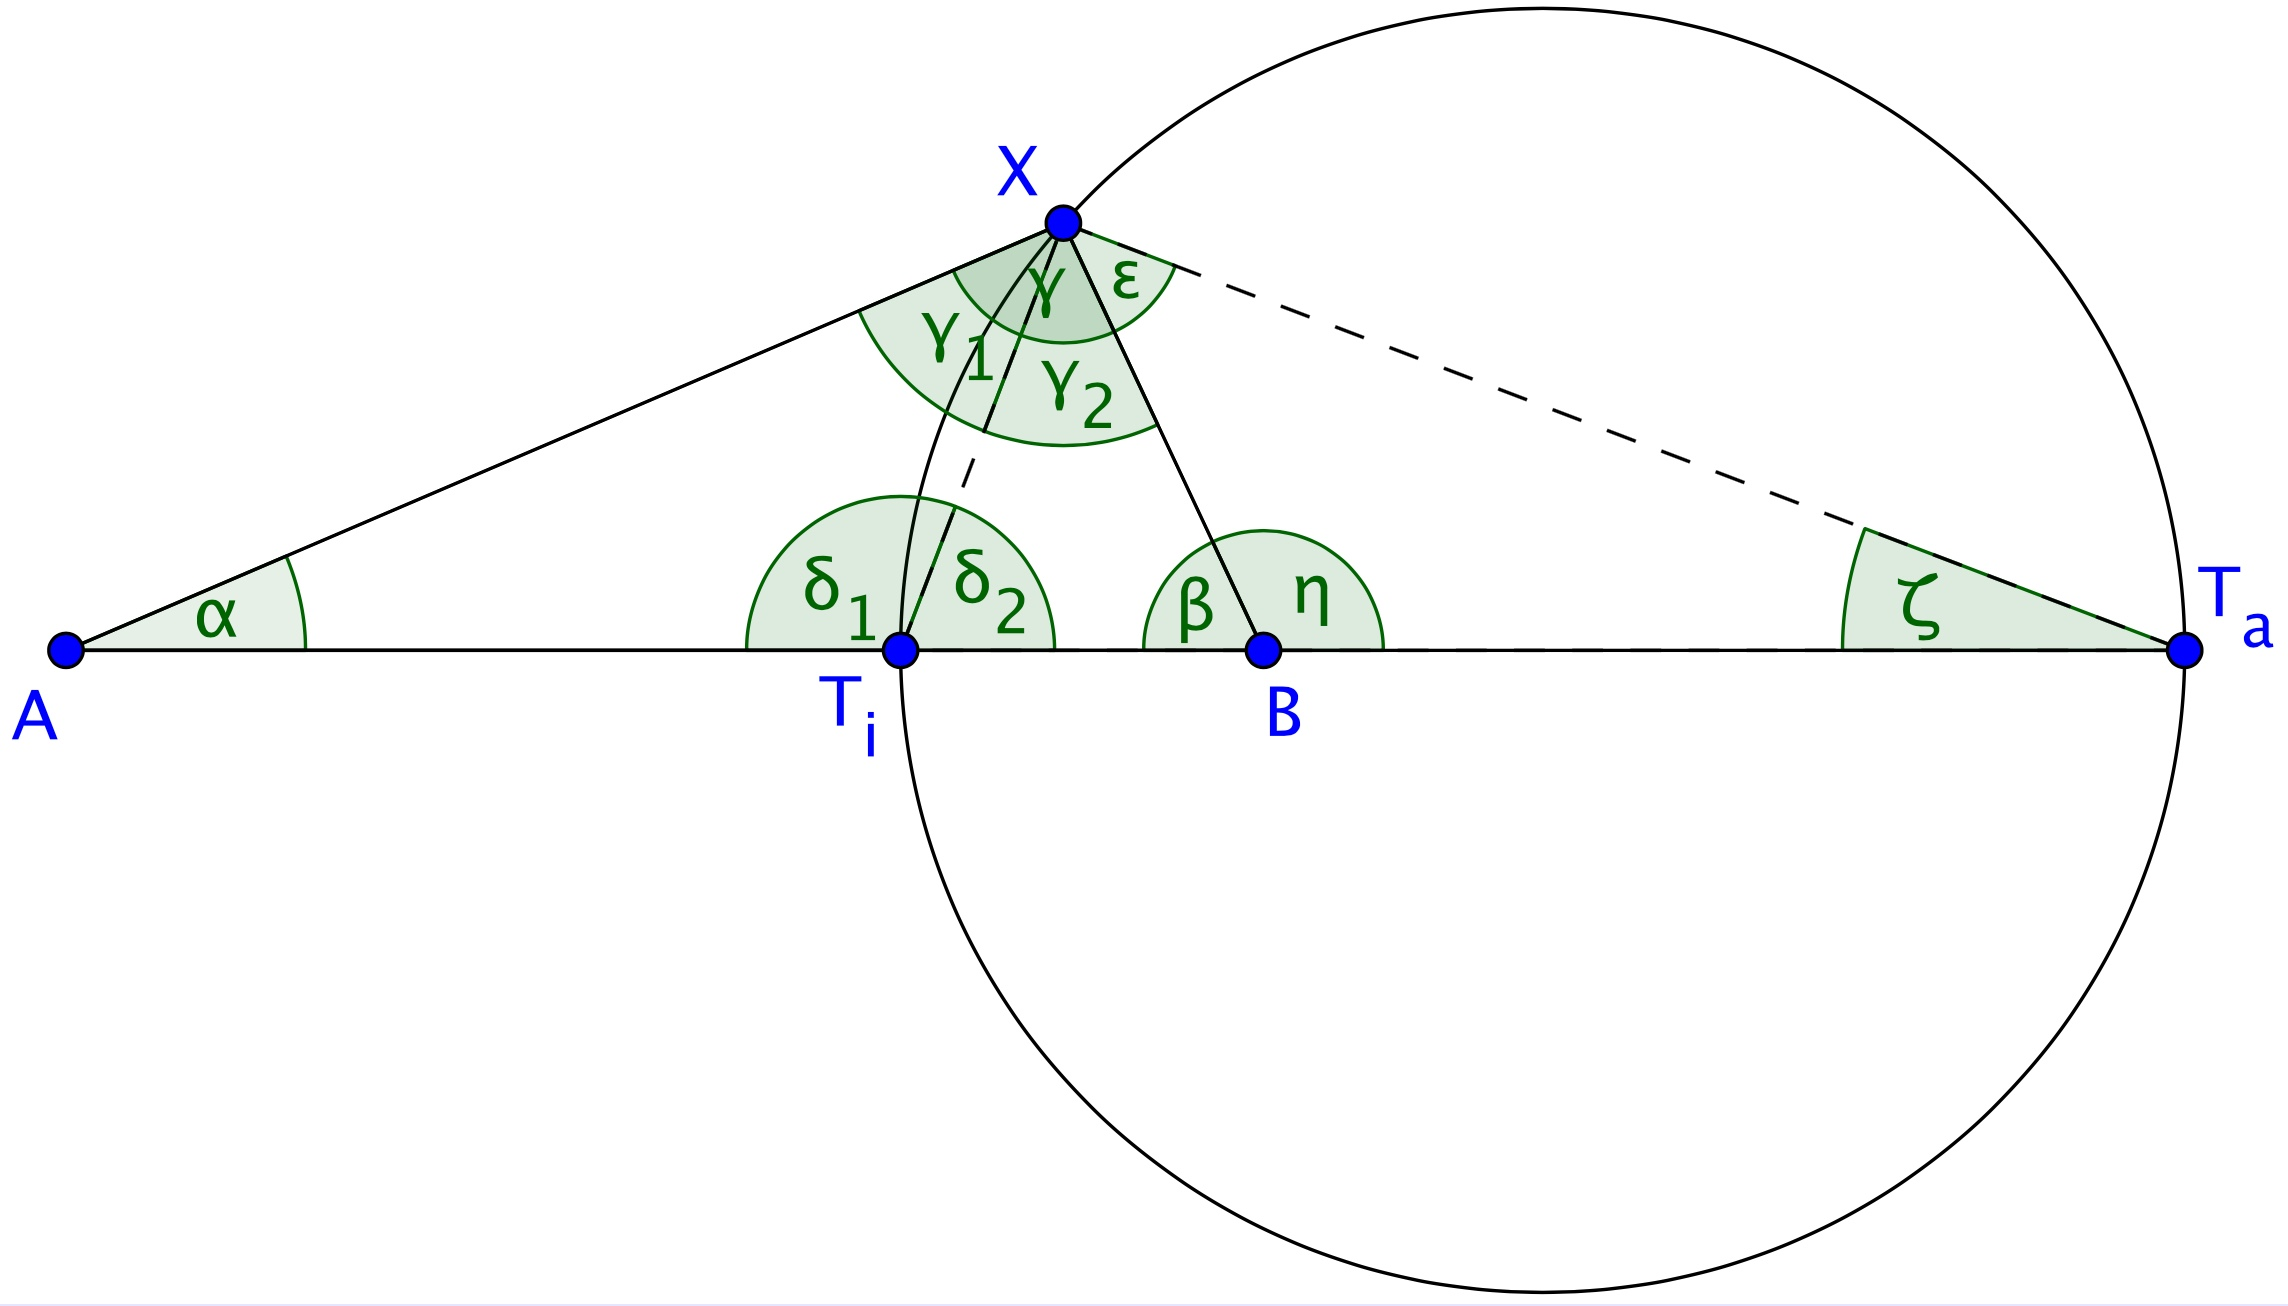
\includegraphics[width=8cm]{kap5/Apollinius_Winkel}
  \end{minipage}
  \begin{minipage}{0.5\textwidth}
    Die Figur und die Zusammenh"ange, die man durch den Satz des Apollinius erhalten hat, kann man benutzen, um ein wenig mit Winkeln zu spielen:
  \end{minipage}\\
  Über diese 10 Winkel lassen sich einige Beziehungen aufstellen:\\
  \begin{array}{rcccl}
  $\vartriangleright \alpha + \beta + \gamma = 180 $ & $\vartriangleright \beta + \gamma_{2} + \delta_{2} = \ang{180} $ & $\vartriangleright \delta_{1} + \delta_{2} = \ang{180} $ & $\vartriangleright \alpha + \gamma + \epsilon + \zeta = \ang{180} $ &$\vartriangleright \epsilon + \zeta + \eta = \ang{180}$\\
  $\vartriangleright \aplha + \gamma_{1} + \delta_{1} = \ang{180} $ & $\vartriangleright \gamma_{1} + \gamma_{2} = \gamma $ & $\vartriangleright \gamma_{2} + \epsilon = \ang{90} $ & $\vartriangleright \beta + \eta = \ang{180} $ &$\vartriangleright \gamma_{2} + \delta_{2} + \epsilon + \zeta = \ang{180}$
  \end{array}
  \\
  Löst man dieses Gleichungssystem, erhält man $\gamma_{1} = \gamma_{2}$, was bedeutet, dass die Gerade $T_{i}X$ Winkelhalbierende des Winkels $\gamma = \angle AXB$ ist:
\end{Bemerkung}
\end{small}

